%%%%%%%%%%%%%%%%%%%%%%%%%%%%%%%%%%%%%%%%%%
%                                        %
% Szablon pracy dyplomowej inzynierskiej % 
%                                        %
%%%%%%%%%%%%%%%%%%%%%%%%%%%%%%%%%%%%%%%%%%



\documentclass[a4paper,twoside,12pt]{book}
\usepackage[utf8]{inputenc}                                      
\usepackage[T1]{fontenc}  
\usepackage{amsmath,amsfonts,amssymb,amsthm}
\usepackage[british,polish]{babel} 
\usepackage{indentfirst}
\usepackage{lmodern}
\usepackage{graphicx} 
\usepackage{hyperref}
\usepackage{booktabs}
\usepackage{tikz}
\usepackage{pgfplots}
\usepackage{mathtools}
\usepackage{geometry}
\usepackage[export]{adjustbox}
\usepackage{multirow}
\usepackage{subcaption}


%\usepackage[nolists,nomarkers]{endfloat}  // wersja pracy z rysunkami i tabelami na końcu
\usepackage[page]{appendix} % toc,
\renewcommand{\appendixtocname}{Dodatki}
\renewcommand{\appendixpagename}{Dodatki}
\renewcommand{\appendixname}{Dodatek}

\usepackage{setspace}
\onehalfspacing


\frenchspacing

\usepackage{listings}
%\lstset{
%	language={},
%	basicstyle=\ttfamily,
%	keywordstyle=\lst@ifdisplaystyle\color{blue}\fi,
%	commentstyle=\color{gray}
%}

%%%%%%%%%%%%%%%%%%%%%%%%%%%
% listingi 
\usepackage{listings}
\lstset{%
language=C++,%
commentstyle=\textit,%
identifierstyle=\textsf,%
keywordstyle=\sffamily\bfseries, %\texttt, %
%captionpos=b,%
tabsize=3,%
frame=lines,%
numbers=left,%
numberstyle=\tiny,%
numbersep=5pt,%
breaklines=true,%
morekeywords={descriptor_gaussian,descriptor,partition,fcm_possibilistic,dataset,my_exception,exception,std,vector},%
escapeinside={@*}{*@},%
%texcl=true, % wylacza tryb verbatim w komentarzach jednolinijkowych
}
%%%%%%%%%%%%%%%%%%%%%%%%%%%%%%%%%%%%


%%%%%%%%%

%%%% TODO LIST GENERATOR %%%%%%%%%

%\usepackage{tikz}
%\usepackage{manfnt}   % dangerous sign 
\usepackage{color}
\definecolor{brickred}      {cmyk}{0   , 0.89, 0.94, 0.28}

\makeatletter \newcommand \kslistofremarks{\section*{Uwagi} \@starttoc{rks}}
  \newcommand\l@uwagas[2]
    {\par\noindent \textbf{#2:} %\parbox{10cm}
{#1}\par} \makeatother


\newcommand{\ksremark}[1]{%
{%\marginpar{\textdbend}
{\color{brickred}{[#1]}}}%
\addcontentsline{rks}{uwagas}{\protect{#1}}%
}

\newcommand{\comma}{\ksremark{przecinek}}
\newcommand{\nocomma}{\ksremark{bez przecinka}}
\newcommand{\styl}{\ksremark{styl}}
\newcommand{\ortografia}{\ksremark{ortografia}}
\newcommand{\fleksja}{\ksremark{fleksja}}
\newcommand{\pauza}{\ksremark{pauza `--', nie dywiz `-'}}
\newcommand{\kolokwializm}{\ksremark{kolokwializm}}
\newcommand{\twobar}{/\kern-0.2em/}
%%%%%%%%%%%%%% END OF TODO LIST GENERATOR %%%%%%%%%%%

%%%%%%%%%%%% ZYWA PAGINA %%%%%%%%%%%%%%%
% brak kapitalizacji zywej paginy
\usepackage{fancyhdr}
\pagestyle{fancy}
\fancyhf{}
\fancyhead[LO]{\nouppercase{\it\rightmark}}
\fancyhead[RE]{\nouppercase{\it\leftmark}}
\fancyhead[LE,RO]{\it\thepage}


\fancypagestyle{tylkoNumeryStron}{%
   \fancyhf{} 
   \fancyhead[LE,RO]{\it\thepage}
}

\fancypagestyle{NumeryStronNazwyRozdzialow}{%
   \fancyhf{} 
   \fancyhead[LO]{\nouppercase{\it\rightmark}}
   \fancyhead[RE]{\nouppercase{\it\leftmark}}
   \fancyhead[LE,RO]{\it\thepage}
}


%%%%%%%%%%%%% OBCE WTRETY  
\newcommand{\obcy}[1]{\emph{#1}}
\newcommand{\ang}[1]{{\selectlanguage{british}\obcy{#1}}}
%%%%%%%%%%%%%%%%%%%%%%%%%%%%%

% polskie oznaczenia funkcji matematycznych
\renewcommand{\tan}{\operatorname {tg}}
\renewcommand{\log}{\operatorname {lg}}

% jeszcze jakies drobiazgi

\newcounter{stronyPozaNumeracja}

\newcommand{\hcancel}[1]{%
    \tikz[baseline=(tocancel.base)]{
        \node[inner sep=0pt,outer sep=0pt] (tocancel) {#1};
        \draw[red] (tocancel.south west) -- (tocancel.north east);
    }%
}%

\newcommand{\miesiac}{%
  \ifcase\the\month
  \or styczeń% 1
  \or luty% 2
  \or marzec% 3
  \or kwiecień% 4
  \or maj% 5
  \or czerwiec% 6
  \or lipiec% 7
  \or sierpień% 8
  \or wrzesień% 9
  \or październik% 10
  \or listopad% 11
  \or grudzień% 12
  \fi}


%%%%%%%%%%%%%%%%%%%%%%%%%%%%%%%%%%%%%%%%%%%%%%
% Helvetica font macros for the title page:
\newcommand{\headerfont}{\fontfamily{phv}\fontsize{18}{18}\bfseries\scshape\selectfont}
\newcommand{\titlefont}{\fontfamily{phv}\fontsize{18}{18}\selectfont}
\newcommand{\otherfont}{\fontfamily{phv}\fontsize{14}{14}\selectfont}

%%%%%%%%%%%%%%%%%%%%%%%%%%%%%%%%%%%%%%%%%%%%%%
%%%%%%%%%%%%%%%%%%%%%%%%%%%%%%%%%%%%%%%%%%%%%%
%%%%%%%%%%%%%%%%%%%%%%%%%%%%%%%%%%%%%%%%%%%%%%
%%%%%%%%%%%%%%%%%%%%%%%%%%%%%%%%%%%%%%%%%%%%%%
%%%%%%%%%%%%%%%%%%%%%%%%%%%%%%%%%%%%%%%%%%%%%%
%%%%%%%%%%%%%%%%%%%%%%%%%%%%%%%%%%%%%%%%%%%%%%
%%%%%%%%%%%%%%%%%%%%%%%%%%%%%%%%%%%%%%%%%%%%%%
%\graphicspath {./images/} 
\newcommand{\autor}{Mikołaj Habarta}
\newcommand{\promotor}{dr hab. inż.  Michał Kawulok}
\newcommand{\konsultant}{}
\newcommand{\tytul}{Narzędzie do ekstrakcji cech głębokich za pomocą konwolucyjnych sieci neuronowych}
\newcommand{\polsl}{Politechnika Śląska}
\newcommand{\wydzial}{Wydział Automatyki, Elektroniki i Informatyki}


\begin{document}
%\kslistofremarks 
	
%%%%%%%%%%%%%%%%%%  STRONA TYTULOWA %%%%%%%%%%%%%%%%%%%
\pagestyle{empty}
{
	\newgeometry{top=2.5cm,%
	             bottom=2.5cm,%
	             left=3cm,
	             right=2.5cm}
	\sffamily
	\rule{0cm}{0cm}
	
	\begin{center}
	
\includegraphics[width=0.4\textwidth]{politechnika_sl_logo_bw_poziom_pl.eps}
	\end{center} 
	\vspace{1cm}
	\begin{center}
	\headerfont \polsl
	\end{center}
	\begin{center}
	\headerfont \wydzial
	\end{center}
	\vfill
	\begin{center}
	\titlefont Praca inżynierska
	\end{center}
	\vfill
	
	\begin{center}
	\otherfont \tytul\par
	\end{center}
	
	\vfill
	
	\vfill
	 
	\noindent\vbox
	{
		\hbox{\otherfont autor: \autor}
		\vspace{12pt}
		\hbox{\otherfont kierujący pracą: \promotor}
		%\vspace{12pt}  % zakomentuj, jezeli nie ma konsultanta
		%\hbox{\otherfont konsultant: \konsultant} % zakomentuj, jezeli nie ma konsultanta
	}
	\vfill 
 
   \begin{center}
   \otherfont Gliwice,  \miesiac\ \the\year
   \end{center}	
	\restoregeometry
}
  

\cleardoublepage
 

\rmfamily
\normalfont

%%%%%%%%%%%%%%%%%%%%% oswiadczenie o udostępnianiu pracy dyplomowej %%%%%%%%%%%%%%%%%%%
\cleardoublepage

\begin{flushright}
załącznik nr 2 do zarz. nr 97/08/09 
\end{flushright}

\vfill  

\begin{center}
\Large\bfseries Oświadczenie
\end{center}

\vfill

Wyrażam  zgodę / Nie wyrażam zgody*  na  udostępnienie  mojej  pracy  dyplomowej / rozprawy doktorskiej*.

\vfill

Gliwice, dnia \today

\vfill

\rule{0.5\textwidth}{0cm}\dotfill 

\rule{0.5\textwidth}{0cm}
\begin{minipage}{0.45\textwidth}
{\begin{center}(podpis)\end{center}}
\end{minipage} 

\vfill

\rule{0.5\textwidth}{0cm}\dotfill 

\rule{0.5\textwidth}{0cm}
\begin{minipage}{0.45\textwidth}
{\begin{center}\rule{0mm}{5mm}(poświadczenie wiarygodności podpisu przez Dziekanat)\end{center}}
\end{minipage}


\vfill

* podkreślić właściwe

 


%%%%%%%%%%%%%%%%%%%%% oswiadczenie promotora o spełnieniu wymagań formalnych %%%%%%%%%%%%%%%%%%%
\cleardoublepage

\rule{1cm}{0cm}

\vfill  

\begin{center}
\Large\bfseries Oświadczenie promotora
\end{center}

\vfill

Oświadczam, że praca „\tytul” spełnia wymagania formalne pracy dyplomowej inżynierskiej.

\vfill



\vfill

Gliwice, dnia \today

\rule{0.5\textwidth}{0cm}\dotfill 

\rule{0.5\textwidth}{0cm}
\begin{minipage}{0.45\textwidth}
{\begin{center}(podpis promotora)\end{center}}
\end{minipage} 

\vfill

 

\cleardoublepage


%%%%%%%%%%%%%%%%%% SPIS TRESCI %%%%%%%%%%%%%%%%%%%%%%
\pagenumbering{Roman}
\pagestyle{tylkoNumeryStron}
\tableofcontents

%%%%%%%%%%%%%%%%%%%%%%%%%%%%%%%%%%%%%%%%%%%%%%%%%%%%%
\mainmatter
\pagenumbering{arabic}
\setcounter{stronyPozaNumeracja}{\value{page}}
\pagestyle{NumeryStronNazwyRozdzialow}

%%%%%%%%%%%%%% wlasciwa tresc pracy %%%%%%%%%%%%%%%%%

\chapter{Wstęp}
{Na przestrzeni ostatniej dekady można było zaobserwować gwałtowny rozwój metod w dziedzinie uczenia maszynowego oraz sieci neuronowych. Pomimo pozornej nowości tych technologii, podstawy teoretyczne wielu z nich zostały opracowane już w latach latach 40. zeszłego stulecia \cite{bib:neural1}. Idee te były sukcesywnie rozwijane oraz modyfikowane, lecz ograniczenia sprzętowe oraz trudność w dostępie do danych uniemożliwiały ich realne wykorzystanie. Dopiero na początku zeszłej dekady postępująca cyfryzacja oraz digitalizacja spowodowała znaczny wzrost ilości przechowywanych danych oraz ich większą dostępność. W Tabeli \ref{tab:datasets} pokazano, jak zmieniały się rozmiary wybranych zbiorów danych przeznaczonych do zagadnień związanych z rozpoznawaniem rysów twarzy na przestrzeni lat. Łatwo zauważyć szybko zwiększające się rozmiary kolejnych baz danych, ze szczególnie gwałtownym wzrostem pomiędzy 2008 a 2014 rokiem. Dzięki dostępności coraz to większych zbiorów danych, ciągle rosnącej mocy obliczeniowej komputerów, oraz technologiach takich jak CUDA (and. \ang {Compute Unified Device Architecture}), które umożliwiają łatwe wykorzystanie tej mocy, systemy oparte na sztucznej inteligencji osiągają coraz to lepsze wyniki i są w stanie wykonywać pewne zadania lepiej niż człowiek.}

{ W ostatnich latach można zaobserwować zwiększający się wpływ tych systemów na ludzkie życie w wielu różnych dziedzinach, takich jak np. diagnostyce chorób, pojazdach autonomicznych, cyberbezpieczeństwie, czy marketingu. Stosunkowo niedawne odkrycia\cite{bib:cancer,bib:cancer2} sugerują, że sztuczna inteligencja może być w stanie odciążyć specjalistów w dziedzinie  diagnostyki chorób nowotworowych, a w przyszłości nawet w pewnym stopniu ich zastąpić. Warto tu również przytoczyć najnowszy przykład AlphaFold, systemu stworzonego przez Google, opartego o uczenie głębokie, który w październiku 2020 roku rozwiązał jedną z największych zagadek biologii\cite{service2020game}. Program nauczył się przewidywać trójwymiarową budowę białka na podstawie jego sekwencji aminokwasów, co było wyzwaniem dla biologów od 50 lat. Zastosowanie tego programu pozwoliło również przyspieszyć pracę nad powstawaniem szczepionki na COVID-19.}

{Te dotychczasowe osiągnięcia systemów opartych o sztuczną inteligencję oraz potencjał tej dziedziny pozwala przypuszczać, że ich znaczenie w świecie będzie już tylko rosnąć. }
 





\begin{table}
\centering
\caption{Rozmiary zbiorów danych służących do rozpoznawania twarzy na przestrzeni lat}
\begin{tabular}{lll}
\hline
Nazwa & Rok powstania & Liczba obrazów \\
\hline
Yale Face Database\cite{Yale} & 1997 & 165 \\
JAFFE Facial Expression Database\cite{lyons1998coding}  & 1998 &  213 \\
Face Recognition Grand Challenge Dataset\cite{bowyer2006survey} & 2004 & 4007 \\
CASIA 3D Face Database\cite{Cas} & 2007 & 4624 \\
Bosphorus\cite{savran2008bosphorus} &2008& 4652 \\
FaceScrub\cite{ng2014data} & 2014 & 107818 \\
IMDB-WIKI\cite{Rothe-ICCVW-2015} & 2015 & 523051 \\
Aff-Wild \cite{zafeiriou2017aff} & 2017 & $\sim$ 1,250,000 \\
Aff-Wild2 \cite{kollias2019expression} & 2019 &$\sim$ 2,800,000 \\
\hline
\end{tabular}

\label{tab:datasets}
\end{table}  

\section{Cel pracy}
{Celem pracy jest stworzenie uniwersalnego narzędzia, które ma umożliwić ekstrakcję wektorów cech głębokich w postaci serializowanej wraz z przypisanymi do nich etykietami w wybranym przez użytkownika formacie. Ekstrakcja jest dokonywana za pomocą konwolucyjnych sieci neuronowych służących do detekcji obiektów. Narzędzie powinno mieć możliwość wyboru architektury sieci, jak i dodania własnych architektur. Domyślną architekturą systemu, która zostanie zaimplementowana będzie architektura R-CNN. Narzędzie ma mieć możliwość użycia własnego zestawu danych w formacie PASCAL-VOC.}
\section{Zakres pracy}
{Zakres pracy obejmuje zgłębienie dziedziny wizji komputerowej oraz przegląd literatury technicznej. Kolejnym krokiem jest zrozumienie konwolucyjnych sieci neuronowych oraz modeli ich wykorzystujących do detekcji obiektów w obrazach, a następnie zapoznanie się bazą danych PASCAL-VOC oraz formatem przechowywanych tam danych. Kolejnym etapem jest przegląd oraz wybór odpowiedniej technologii, a następnie spisanie wymagań pracy oraz implementacja. }
\section{Plan pracy}
{Praca składa sie z 7 rozdziałów, które opisują teoretyczne oraz praktyczne ujęcie tematu.}

{Rozdział 1 zawiera wstęp do tematu oraz określenie celów projektu.}

{Rozdział 2 składa się z analizy zagadnienia detekcji obiektów w obrazach, przeglądu i porównanie dotychczas znanych rozwiązań i technologii.}

{W rozdziale 3 omówiono wymagania funkcjonalne i niefunkcjonalne oraz dokonano opisu zastosowanych narzędzi.}

{Rozdział 4 obejmuje specyfikacje zewnętrzną. Zostanie w nim opisany sposób instalacji oraz przykładowe scenariusze korzystania z narzędzia.}

{W rozdziale 5 można znaleźć opis architektury systemu oraz omówienie użytych modułów i bibliotek.}

{Rozdział 6 zawiera opis weryfikacji oraz walidacji systemu.}

{W rozdziale 7 zawarto podsumowanie całej pracy oraz wnioski z niej płynące. Wymieniono również największe trudności, które napotkano w czasie pracy nad projektem.}

%\begin{itemize}
%\item wprowadzenie w problem/zagadnienie
%\item osadzenie problemu w dziedzinie
%\item cel pracy
%\item zakres pracy
%\item zwięzła charakterystyka rozdziałów
%\item jednoznaczne określenie wkładu autora, w przypadku prac wieloosobowych – tabela z autorstwem poszczególnych elementów pracy
%\end{itemize}


\chapter{Analiza dziedziny}
{W tym rozdziale zostanie omówiony problem detekcji oraz klasyfikacji obiektów w obrazach. Pokrótce wyjaśniona zostanie zasada działania konwolucyjnych sieci neuronowych, ze zwięzłym opisem różnych rodzajów warstw, a następnie przedstawione zostanie kilka najważniejszych modeli sieci neuronowych. Opisana zostanie architektura R-CNN, która została zaimplementowana w programia, oraz algorytm wyszukiwania selektywnego, który również został zaimplementowany w ramach tej architektury. Aby móc uzyskać jakieś porównanie co do wydajności i ograniczeń architektury R-CNN,  pokazane zostaną również inne architektury sieci, takie jak Fast R-CNN czy YOLO.}

\section{Analiza problemu}
{Człowiek postrzega świat głównie wizualnie. Szacuje się, że 80 \% bodźców odbieranych przez człowieka to bodźce wzrokowe. Niektóre z teorii \cite{nilsson2013eye} pozwają przypuszczać, że wykształcenie oka było najważniejszym momentem w historii ewolucji oraz kluczowym elementem, który umożliwił powstanie inteligentnych form życia. Nic więc dziwnego, że temat tak znaczący dla człowieka otrzymuje proporcjonalnie dużo uwagi w dziedzinie sztucznej inteligencji. Umożliwienie maszynom zrozumienia wizualnych danych jest głównym celem, do którego spełnienia jesteśmy, zdawać by się mogło, coraz bliżej.}

{Jednym z podstawowych problemów z dziedziny wizji komputerowej jest klasyfikacja. Polega ona na przypisaniu pewnej kategorii na podstawie obrazu. Zazwyczaj kategorie te to obiekty znajdujące się na zdjęciu. Chcemy więc, aby maszyna po zobaczeniu zdjęcia zawierającego jakiś obiekt  psa skategoryzowała go jako 'pies'. Do problemu klasyfikacji możemy dołożyć jeszcze inny problem – detekcji. W ramach tego problemu oczekujemy, aby maszyna bo zobaczeniu jakiegoś zdjęcia zidentyfkowała wszystkie obiekty, które się na nim znajdują, oraz wskazała w którym miejscu na zdjęciu te obiekty się znajdują.}
\section{Sztuczne sieci neuronowe}
{Podstawą budowy sieci neuronowej jest węzeł\cite{bishop1995neural}, nazywany też czasem neuronem. Każdy węzeł ma swoje parametry – wagi. Każdy neuron przyjmuje pewne dane wejściowe oraz wytwarza dane wyjściowe, obydwa o stałym rozmiarze. Nauka sieci neuronowej polega na dobraniu odpowiednich parametrów za pomocą propagacji wstecznej dla każdego z neuronów tak, aby sieć na wyjściu zwracała oczekiwany rezultat\cite{8118}. Neurony grupuje się w warstwy, które łączy się ze sobą. Na rysunku \ref{simplenetwork} przedstawiono prosty model sieci neuronowej, w którym każdy neuron jest połączony ze wszystkimi neuronami z następnej warstwy. Taki rodzaj warstw nazywa się warstwą w pełni połączoną, lub gęstą, a sieci stworzone z takich warstw sztucznymi sieciami neuronowymi. Taki model sieci otrzymuje dane wejściowe o stałym rozmiarze oraz produkuje dane wyjściowe o stałym rozmiarze. W przypadku problemu klasyfikacji danymi wejściowymi jest obraz, a danymi wyjściowymi – klasa obiektu. Ponieważ na wyjściu sieci otrzymujemy liczbę (wektor), to stosuje się kodowanie 1 z n, aby zamienić otrzymany wynik na odpowiednią klasę.

\begin{figure}[h!]


\centering
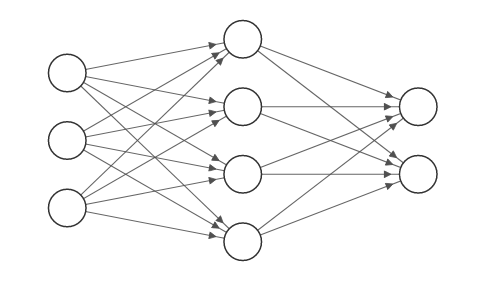
\includegraphics[scale=0.75]{connected.png}
\caption{Przykład prostej sieci w pełni połączonej}
\label{simplenetwork}
\end{figure}




\subsection{Konwolucyjne sieci neuronowe}{Sztuczne sieci neuronowe dominowały w początkowych latach badań, jednak wraz z rozwojem dziedziny opracowano inne modele sieci, które miały służyć już bardziej konkretnym zadaniom. Modelem, który został stworzony do analizowania scen wizualnych był model konwolucyjny, nazywany też splotowym. }
{Inspiracją do stworzenia tego modelu były odkrycia neurofizjologów Hubela i Wiesela z lat 50. i 60. zeszłego wieku. \cite{hubel1959receptive,hubel1963shape,hubel1968receptive} Odkryli oni, że neurony w korze wzrokowej reagują na określone pole widzenia. Każdy neuron ma swoje pole recepcyjne i reaguje na bodziec tylko w obrębie tego pola. Sieci konwolucyjne starają się odzworować sposób działania tych neuronów w korze wzrokowej. Zamiast patrzeć na obraz jako całość, każdy neuron jest odpowiedzialny za jego małą część. Neurony posiadające pole recepcyjne nazywa się kernelami, albo filtrami, gdyż działają dokładnie jak klasyczne filtry, a warstwę filtrów nazywa się warstwą konwolucyjną. Sieci konwolucyjne składają się zazwyczaj z wielu warstw konwolucyjnych, przeplatanych innymi warstwami (np. próbkującymi), a na ich końcach umieszcza się jedną lub kilka warst w pełni połączonych. Zadaniem tych warstw w pełni połączonych jest dokonanie klasyfikacji na podstawie wyjścia z ostatniej warsty konwolucyjnej. To właśnie wyjście z ostatniej warstwy konwolucyjnej nazywane jest wektorem cech głębokich. Poniżej zostanie dokonany dokładniejszy opis warstwy konwolucyjnej, jak i również kilku innych rodzajów warstw, które są powszechnie używane w sieciach neuronowych.}

\subsubsection{Warstwa konwolucyjna}
{Warstw konwolucyjna to zbiór kerneli (filtrów), zawierających parametry, które należy nauczyć. Kernele są zazwyczaj małych rozmiarów, mniejszych od rozmiaru obrazu wejściowego. Typowym rozmiarem kernela jest np. $3 \times 3 \times3$, który oznacza, że pokrywa on obszar 3 na 3 piksele, uwzględniając 3 wymiary RGB odpowiadajace za barwę. Filtr jest następnie przesuwany przez cały obraz wejściowy, i w każdej jego pozycji obliczany jest iloczyn skalarny między nim a danymi wejściowymi, co przedstawia rysunek \ref{conv1}. W wyniku tego działania otrzymujemy pewną macierz, która nazywa się mapą aktywacji danego kernela. Mapy aktywacji wszystkich filtrów z danej warstwy są nakładane na siebie i tworzą trójwymiarową macierz, która jest podawana na wyjściu warstwy konwolucyjnej, co pokazano na rysunku \ref{conv2}.}

\begin{figure}[h!]
\centering
 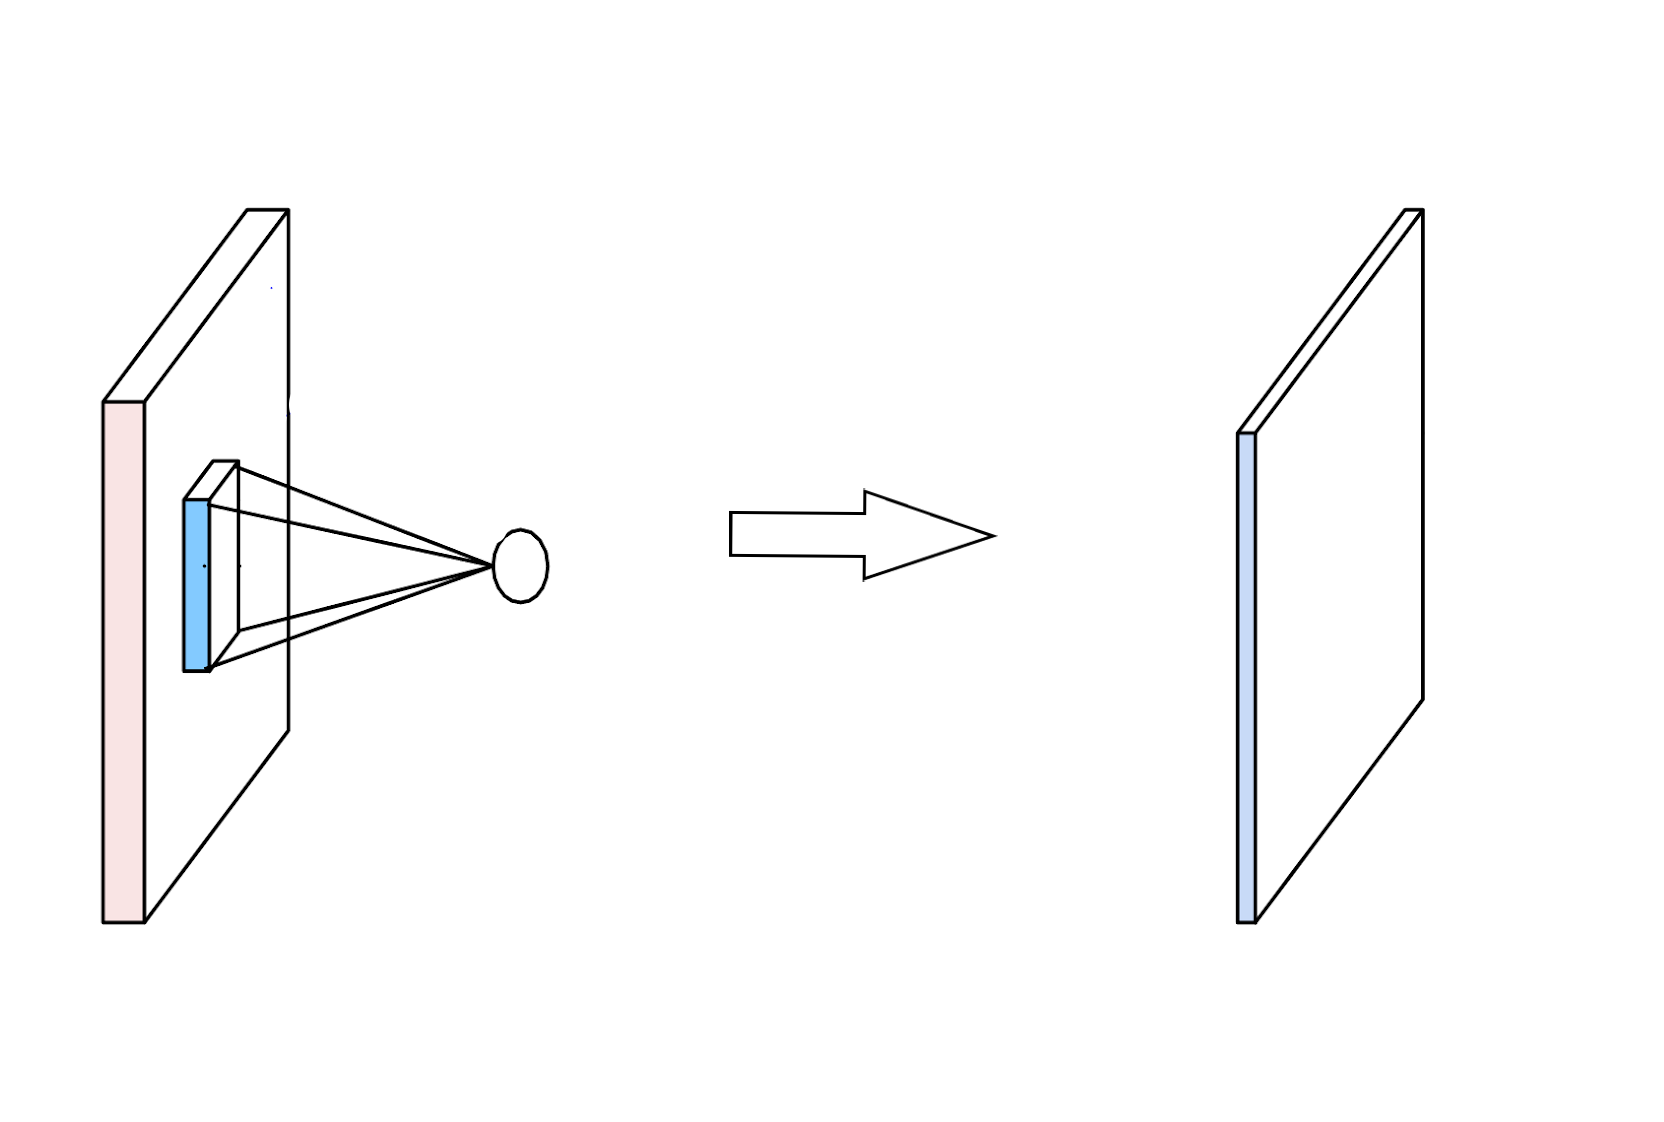
\includegraphics[scale=0.20]{conv1.png}
  \caption{Filtr o wymiarach 5x5x3}
\label{conv1}
\end{figure}

\begin{figure}[h!]
  \centering
  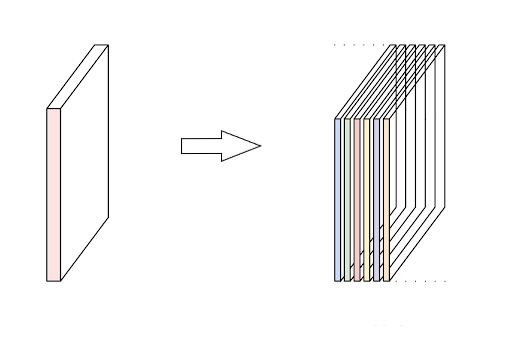
\includegraphics[scale=0.7]{conv2.png}
  \caption{Mapy aktywacji nakładane na siebie}
  \label{conv2}

\end{figure}






\subsubsection{Warstwa próbkująca}
{Nazywana też czasem warstwą łączenia(ang. \ang {pooling layer}), najczęściej umieszczana jest pomiędzy dwoma warstwami konwolucyjnymi. Jej zadaniem jest redukcja rozmiaru otrzymanych map aktywacji, co zmiejsza ilosć parametrów, których sieć musi się nauczyć. Ta warstwa opiera się u filtry najczęściej o rozmiarach $2\times2$, które biorą maksymalną lub średnią wartość z każdego rejonu i zmniejszają w ten sposób wysokość oraz szerokość danych, nie zmieniając jednak głębokości.}


\subsubsection{Warstwa aktywacyjna}
{Ta warstwa to funkcja matematyczna, która decyduje o tym, czy neuron ma być aktywny, czy nie, na podstawie jego wartości. Powinna być to funkcja szybka do obliczenia, bo będzie wykonywana dla każdego nueronu w sieci. Początkowo często używaną funkcją był $\tanh(x)$ (rys. \ref {tanh}) , ale z czasem okazało się że funkcja rektyfikowanej jednostki liniowej (ReLU), definiowanej jako $\max(0,x)$(rys. \ref{ReLu}) pozwala osiagnąć lepsze wyniki \cite{nair2010rectified,glorot2011deep} i aktualnie jest najczęściej używaną funkcją aktywacji \cite{ramachandran2017searching}.}



\begin{figure}
\centering
\begin{subfigure}{.5\textwidth}
  \centering
  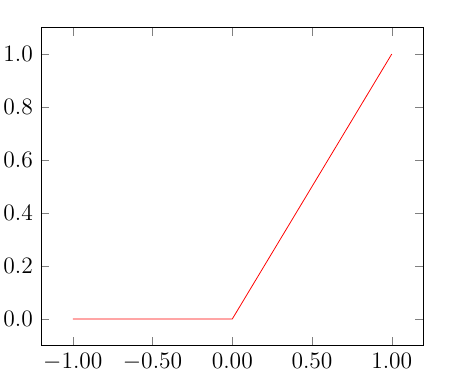
\includegraphics[width=.8\linewidth]{relu.png}
  \caption{ReLU}
  \label{ReLu}
\end{subfigure}%
\begin{subfigure}{.5\textwidth}
  \centering
  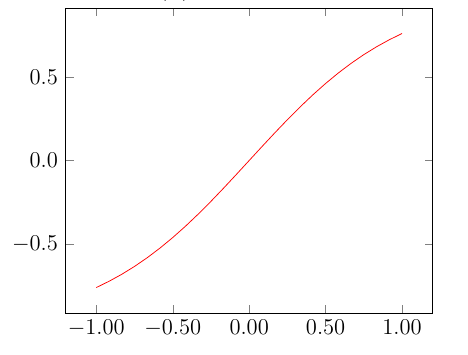
\includegraphics[width=.8\linewidth]{tanges.png}
  \caption{Tangens hiperboliczny}
  \label{tanh}
\end{subfigure}
\caption{Funkcje aktywacji.}
\end{figure}


\subsubsection{Warstwa normalizująca}
{Warstwa ta została zaproponowana w celu zmiejszenia złożoności obliczeniowej poprzez normalizację aktywacji neuronów \cite{ba2016layer}, jednak doświadczenia praktyczne sugerują, że ich wpływ jest znikomy, przez co stosowane są bardzo rzadko i tylko w kontretnych przypadkach.}

\subsubsection{Warstwa regularyzacji opuszczeń}
{Warstwa ta w sposób losowy wyłącza pewną część neuronów (najczęściej 50\%), poprzez ustawienie ich wartości na 0, co sprawia, że nie będą aktywne. Może wydawać się to nieintuicyjne, jednak ta technika sprawia, że sieć musi być bardziej elastyczna i nie może zawsze polegać na istniejących już połączeniach. Pozwala do zapobiegać nadmiernemu dopsowaniu sieci oraz sprawia, że sieć osiąga lepsze rezultaty \cite{srivastava2014dropout,dahl2013improving,hinton2012improving}.}

\subsection{Przykładowe modele sieci}
{Na przestrzeni lat pojawiło się kilka modeli sieci neuronowych, które, czy to ze względu na swoją innowacyjność, czy na uzyskiwane wyniki, miały wielki wpływ na rozwój dziedziny i są powszechnie znane w środowiskach naukowach.}
\subsubsection{LeNet}
{Jest to pierwsza udana implementacja konwolucyjnej sieci neuronowej. Stworzona w latach 90. przez Yanna LeCuna służyła do rozpoznawania ręcznie pisanych cyfr z kodów pocztowych\cite{lecun1998gradient}. Składała się z 3 warstw konwolucyjnych na przemian z warstwami próbkującymi, oraz z jednej warstwy w pełni połączonej na samym końcu, co pokazano na rysunku \ref{LeNet}. }

\begin{figure}[h]


\centering
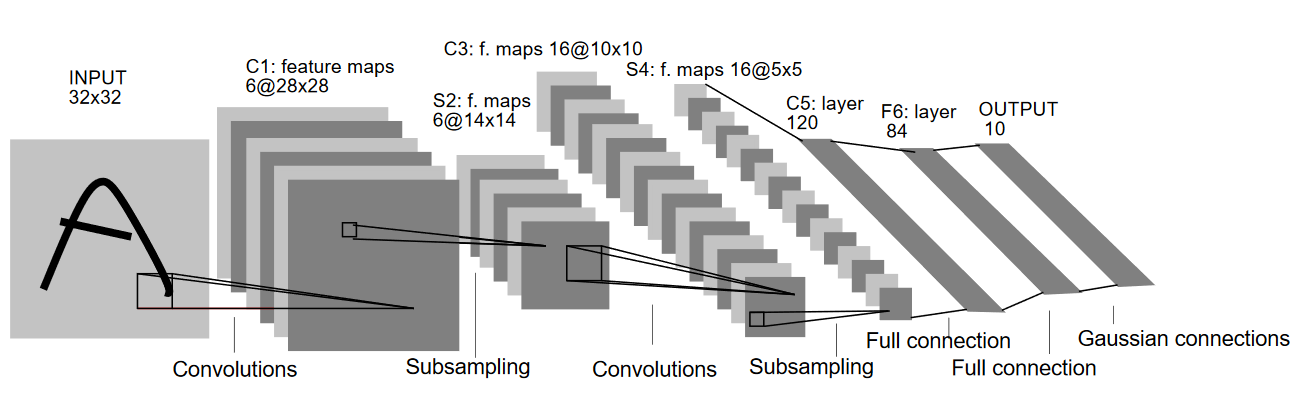
\includegraphics[scale=0.6]{le-net-5.png}
\caption{Architektura sieci LeNet (źródło: \cite{lecun1998gradient})}
\label{LeNet}
\end{figure}

\subsubsection{AlexNet}
{Sieci konwolucyjne zyskały popularność w latach 90., jednak wymagały dużej mocy obliczeniowej, które przy ówczesnym poziomie techniki były trudno dostępne (warto przypomnieć, że technologia CUDA powstała dopiero w 2007 roku), przez co wypadły z łask na rzecz maszyn wektorów nośnych\cite{girshick2014rich}. Sytuacja ta utrzymywała się aż to 2012 roku, kiedy to Alex Krizhevsky i in. stworzyli sieć AlexNet\cite{krizhevsky2012imagenet}. Sieć osiągnęła najlepszy rezultat w konkursie ILSVRC, z błędem na poziomie 15,3\%, ponad 10 punktów procentowych lepiej od drugiego miejsca. Ten świetny rezultat na nowo pobudził zainteresowanie technologią sieci konwolucyjnych, a sieć ta jest uważana za jedną z najbardziej wpływowych w dziedzinie wizji komputerowej. Używa ona ReLU jako funkcji aktywacji, co nie było standardem w tym czasie. Zastosowana została warstwa regularyzacji opuszczeń z prawdopodobieństwem 50\%, jak i również augmentacja danych, co zmniejszyło nadmierne dopasowanie, a użycie procesorów graficznych pozwoliło na szybsze wykonanie kosztownych obliczeń. Na rysunku \ref{AlexNet} pokazano architekturę sieci AlexNet.}
\begin{figure}[h]


\centering
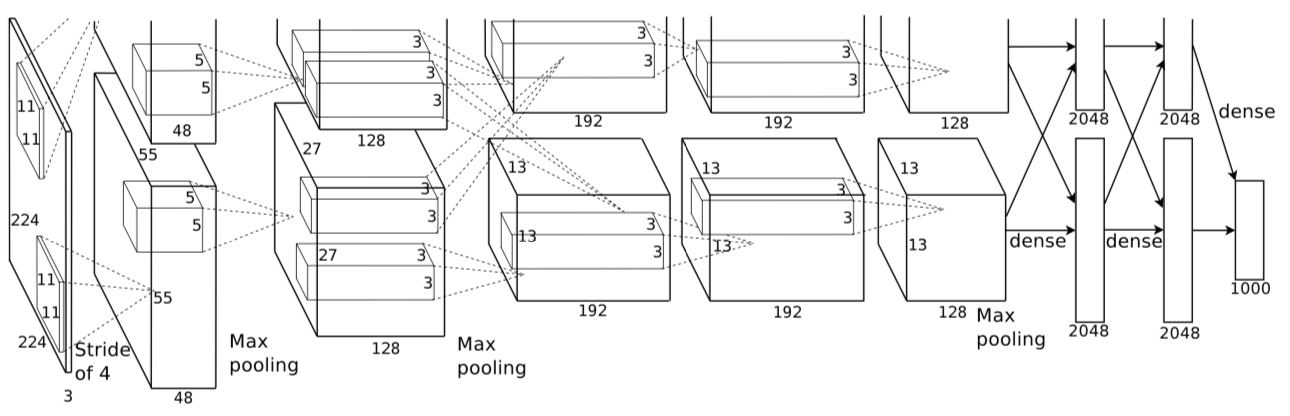
\includegraphics[scale=0.24]{alex.png}
\caption{Architektura sieci AlexNet. Sieć została tutaj podzielona na dwie równoległe części, ponieważ obliczenia były dzielone pomiędzy dwie jednostki graficzne (źródło:\cite{krizhevsky2012imagenet})}
\label{AlexNet}
\end{figure}

\subsubsection{VGG16}
\label{vg}
{Stworzona w 2014 roku przez Simonyana i Zissemana\cite{simonyan2014very}, pomimo tego, że zajęła 2 miejsce w konkursie ILSVRC, jest jedną z najbardziej rozpoznawalnych sieci w dziedzinie. Simonyan i Zisseman przyjęli inną strategii – zamiast zmieniać i testować różne wielkości warstw, użyli w niej warst konwolucyjnych o stałym wymiarze $3\times3$ oraz próbkujących o rozmiarze $2\times2$ , a testowali jedynie różne głębokości sieci. W ramach pracy stworzono kilka wariantów sieci o różnej głębokości. Najlepszy okazał się wariant z 16 warstwami, którego architekturę zaprezentowano na rysunku \ref{VGG}. Ten model pokazał, że głębokość sieci jest kluczowym czynnikiem decydującym o dobrym rezultacie.}
\begin{figure}[h!]


\centering
\includegraphics[scale=0.4]{VGG.png}
\caption{Architektura sieci VGG (źródło: https://stanford-cs221.github.io/autumn2019-extra/posters/101.pdf)}
\label{VGG}
\end{figure}







\subsubsection{ResNet}
\label{Res}
{Sieć ta stworzona została przez Kaiminga He i in. i wygrała konkurs ILSVRC w 2015 roku\cite{he2016deep}. Jest przykładem sieci szczątkowej, w której niektóre połączenia pomiędzy warstwami są pomijane. Takie rozwiązanie pozwala na lepszą skalowalość wraz ze zwiększaniem liczby warstw oraz eliminuje problem tzw. zanikającego gradientu. Sieć ta posiada olbrzymią liczbę 152 warstw, i ta glebokość w połączeniu z nową technologią sprawiła, że przez długi czas była ona szczytowym osiągnięciem technologii.}

\section{R-CNN}
\label{rcnn}
{Zastosowanie konwolucyjnych sieci neuronowych w problemie klasyfikacji jest stosunkowo proste, ponieważ wymiary danych wejściowych oraz wyjściowych są stałe. Jako dane wejściowe przekazywany jest obraz, a jako dane wyjściowe tworzony jest wektor klasyfikujący ten obraz. Co prawda obraz ten może być różnej wielkości, lecz najczęściej skaluje się go do wymaganych rozmiarów. W przypadku detekcji jednak pojawia się problem, ponieważ liczba obiektów na zdjęciach może być różna, więc nasza sieć musiałaby dawać wyniki o zmiennych rozmiarach, co jest sprzeczne z jej zasadą działania. Przykładowo dla obrazu z jednym obiektem sieć powinna zwrócić klasę tego obiektu oraz prostokąt, w którym się znajduje. Ponieważ prostokąt jest opisywany przez cztery wierzchołki, to w tym przypadku oczekiwany jest wyniki w postaci pięciu liczb, lecz jeżeli obiektów będzie więcej, to ilość parametrów potrzebnych do ich opisania będzie odpowiednio większa. Mamy więc do czynienia z sytuacją, gdzie rozmiar danych wyjściowych jest zależny od danych wejściowych. Początkowym rozwiązaniem było użycie okna, które przesuwało się po obrazie w każdej pozycji oraz klasyfikowało zaznaczony obszar \cite{szegedy2013deep}. Okno musiało sprawdzić każdą możliwą lokalizację, dodatkowo musiało zmieniać rozmiar, co skutkowało ogromną ilością obliczeń.}

{W celu rozwiązania tego problemu Ross Girshick i in. zaproponowali w 2014 roku rozwiązanie – regionalną konwolucyjną sieć neuronową\cite{girshick2014rich}. Rozwiązanie to zakłada, że najpierw z obrazu wydzielamy propozycje około 2000 regionów, w których jest duże prawdopodobieństwo, że znajduje się jakiś obiekt. Do wydzielania tych regionów, nazywanych też regionami zainteresowań (\ang {RoI - Regions of Interest}), służy algorytm selektywnej selekcji, opisany dokładniej w podrozdziale \ref{ss}. Następnie każdy z tych regionów służy jako dane wejściowe do konwolucyjnej sieci neuronowej, która wyznacza dla niego wektor cech głębokich. Następnie te wektory poddawane są klasyfikacji. W pierwotnej wersji klasyfikacja ta była przeprowadzana za pomocą maszyny wektorów wspierających, ale można używać innych metod w celu poprawy dokładności sieci.}
\subsection{Miara IoU}
\label{iou}
{Podczas detekcji musimy zmierzyć się z jeszcze jednym zadaniem – musimy zlokalizować nasz obiekt na zdjeciu. Jako lokalizację przyjmuje się wyznaczenie prostokątu, w którym znajduje się obiekt. Pojawia się więc problem, w jaki sposób ocenić, czy wyznaczony przez nas obszar pokrywa się z prostokątem zawierającym obiekt. Nie możemy oczekiwać, że wyznaczymy dokładnie identyczny obszar, ponieważ byłoby to wręcz niemożliwe. Wystarczy nam, że nasz obszar tylko w pewnym stopniu będzie pokrywał prostokąt. W celu ewaluacji tej miary używa się operatora IoU (ang. \ang{Intersection over Union} – przecięcie nad połączeniem), który używa współczynnika matematycznego, zwanego indeksem Jaccarda, definiowanego jako: 

\begin{equation}
F(A,B) = \frac{| A \cap B|}{ |A \cup B|},\\
\end{equation}
czyli iloraz powierzchni wspólnej oraz sumy obu obszarów. Próg, od którego uznajemy, że wyznaczony obszar zawiera obiekt jest wyznaczany umownie (zazwyczaj jest to 0.5), a jego zmiana może znacząco wpływać na wynik sieci \cite{girshick2014rich}. Obszary z miarą IoU powyżej tego progu są uznawane za próbki dodatnie, ponieważ znajdują się w nich jakieś obiekty, a poniżej tego progu – ujemne, czyli zawierające tło.}

\subsection{Algorytm wyszukiwania selektywnego}
\label{ss}
{Algorytm ten~\cite{uijlings2013selective} ma za zadanie wyznaczyć propozycje regionów, które będą później używane do detekcji obiektów. Na początku algorytm dokonuje segmentacji obrazu na podstawie intensywności pikseli, bazując na zaproponowanej przez Felzenszwalba i in. metodzie segmentacji z zastosowaniem teorii grafów \cite{felzenszwalb2004efficient}. Następnie obszary, które są do siebie podobne, są ze sobą łączone. Podobieństwo obszarów określa się na podstawie czterech cech: koloru, tekstury, rozmiaru i kształtu.}
\subsubsection{Podobieństwo koloru}
{Dla każdego regionu generowany jest histogram danego kanału barwy. Wszystkie kanały są następnie zestawiane razem w wektor o określonej długości $n$, a podobieństwo jest wyliczane według wzoru:
\begin{equation}
P_{koloru}(r_{i},r_{j})= \sum_{k=1}^{n} min(c_{i}^k,c_{j}^k),\\
\end{equation}
gdzie $c_{i}^k, c_{i}^k$ są wartością k-tego przedziału histogramu dla regionów kolejno: $r_{i}$ i $r_{j}$.
}
\subsubsection{Podobieństwo tekstury}
{
Dla każdego kanału liczonych jest 8 pochodnych Gaussa przy $\sigma=1$. Na ich podstawie dla każdego regionu tworzony jest histogram, a podobieństwo tekstur jest liczone jako:
\begin{equation}
P_{tekstury}(r_{i},r_{j})= \sum_{k=1}^{n} min(t_{i}^k,t_{j}^k),\\
\end{equation}
gdzie $t_{i}^k,  t_{i}^k$ są wartością k-tego przedziału histogramu dla regionów kolejno: $r_{i}$ i $r_{j}$.

}
\subsubsection{Podobieństwo rozmiaru}
{To podobieństwo premiuje rozwiązania łączące mniejsze regiony, jednocześnie pozwala unikać sytuacji, w której jeden region wchłania wszystkie inne. Dla obrazu o rozmiarze w pikselach $size(im)$ jest ono liczone jako:
\begin{equation}
P_{rozmiaru}(r_{i},r_{j})= 1- \frac{size(r_{i})+size(r_{j})}{size(im)}.\\
\end{equation}}
\subsubsection{Podobieństwo kształu}
{To podobieństwo określa, jak bardzo dwa regiony do siebie pasują. Jest zdefiniowane jako:
\begin{equation}
P_{kształtu}(r_{i},r_{j})= 1- \frac{size(BB_{ij})- size(r_{i})+size(r_{j})}{size(im)},\\
\end{equation}
gdzie $BB_{ij}$ jest obwiednią dookoła regionów $r_{i}$ i $r_{j}$.
}


{Końcowe podobieństwo można uzyskać ze wzoru:
\begin{equation}
P(r_{i},r_{j})= a_{1}P_{koloru}+a_{2}P_{tekstury}+a_{3}P_{rozmiaru}+a_{4}P_{kształtu},\\
\end{equation}
gdzie $a_{i} \in  \{0,1\}$ określa, czy miara podobieństwa jest użyta.
}


\subsection{Wady modelu R-CNN}
{Pomimo swojej użyteczności, model R-CNN nie jest pozbawiony wad. Konieczność wykonania obliczeń dla każdego z 2000 regionów sprawia, że model działa bardzo wolno, przez co wytrenowanie go może zająć duże ilości czasu. Dodatkowo nie może znaleźć on zastosowania w sytuacjach czasu rzeczywistego (np. analiza obrazu z kamery), przetworzenie każdego obrazu zajmuje średnio 40 sekund. Należy też zauważyć, że na etapie wyznaczania regionów nie następuje żadna nauka sieci  –  algorytm wyszukiwania selektywnego jest algorytmem stałym i niezależnym od parametrów sieci. Kolejne rozwiązania starają się rozwiązać te problemy. }
\section{Inne architektury}
\subsubsection{Fast R-CNN}
{Ross Girshick rok po publikacji swojej pracy opisującej R-CNN zaproponował jej ulepszoną wersję – Fast R-CNN\cite{girshick2015fast}. Jak sama nazwa wskazuje, rozwiązanie to jest szybsze od swojej pierwszej wersji. Zamiast wyznaczać dużą liczbę regionów, na których następnie sieć dokonuje obliczeń, w tym modelu przekazujemy wejściowy obraz do sieci konwolucyjnej, a dopiero na otrzymanej z sieci mapie aktywacji dokonujemy podziału na regiony, które następnie klasyfikujemy. Dzięki temu rozwiązaniu znacząco zmniejszamy czas obliczeń, co dla modelu VGG16 oraz zbioru danych PASCAL VOC 2012 skutkuje 9-krotnym przyspieszeniem etapu treningu sieci oraz aż 213-krotnym przyspieszniem etapu testowania, przy jednoczesnym zwiększeniu precyzji sieci.}
\subsubsection{Faster R-CNN}
{Wszystkie poprzednie metody używały algorytmu wyszukiwania selektywnego do wyznacznia propozycji regionów, jednak wraz ze wzrostem szybkości innych elementów modelu, ten algorytm stał się ,,wąskim gardłem'' obliczeniowym, dlatego postanowiono z niego zrezygnować. W ten sposób powstała architekura Faster R-CNN~\cite{ren2015faster}, jeszcze szybsza od swoich poprzedniczek, w której propozycje regionów są wyznaczane również przez równoległą sieć neuronową. Dzięki temu udało się jeszcze bardziej przyspieszyć działanie sieci – autorzy tego rozwiązania osiągali wyniki rzędu 200 ms na obraz.}
\subsubsection{YOLO}
{Architektura YOLO (\ang{You Only Look Once} – patrzy się tylko raz) stara się traktować problem detekcji jako problem regresji~\cite{redmon2016you}. Zamiast na cały obraz, sieć patrzy tylko na te fragmenty, w których jest bardziej prawdopodobne, że występuje jakiś obiekt. Wszystkie zadania – lokalizację obiektów oraz klasyfikację wykonuje tylko jedna sieć, co drastycznie zwiększa szybkość tego rozwiązania, pozwalając na zastosowanie go w celu detekcji w czasie rzeczywistym (w artykule proponującym to rozwiązanie autorzy chwalą się osiągnięciem 45 klatek na sekundę). Wadą tego rozwiązania jest mniejsza precyzja sieci – często pomija obiekty, szczególnie jeżeli są dość małe.}


 
\chapter{Wymagania i narzędzia}
{W tym rozdziale zostanie dokonany opis wymagań funkcjonalnych oraz niefunkcjonalnych pracy oraz zaprezentowane zostaną diagramy przypadków użycia. Następnie omówione będą użyte narzędzia oraz opisana zostania metodyka pracy nad projektowaniem i implementacją.}
\section{Wymaganie funkcjonalne i niefunkcjonalne}
\subsection{Wymagania funkcjonalne}
{Projekt powinien realizować następujące funkcjonalności:
\begin{itemize}
\item{Użytkownik powinien móc dokonać wyboru architektury sieci.}
 \item {Powinna istnieć możliwość łatwego dodania innych architektur sieci.}
 \item{W ramach architektury, użytkownik ma mieć możliwość wczytania swojego modelu z pliku, wyświetlenia listy dostępnych modeli oraz wyboru modelu sieci.}
  \item {Dla określonych danych wejściowych, program ma mieć możliwość zapisania cech głębokich ekstrahowanych przez sieć, wraz z odpowiadającymi im etykietami. Poprzez cechy głębokie rozumie się ostatnią warstwę sieci konwolucyjnej, którą sieć oblicza przed dokonaniem klasyfikacji. }
  \item{Użytkownik ma mieć możliwość wyboru formatu, w którym zostaną zapisane (tekst lub hdf5).}
  \item{Powinna istnieć możliwość wyboru dowolnych danych wejściowych, zgodnych z formatem PASCAL VOC, i to na tych danych zostanie wykonana ekstrakcja.}
  \item{Powinna istnieć możliwość wybrania klas, dla których zostanie dokonana ekstrakcja.}
  \item{W ramach projektu zostanie zaimplementowana architektura R-CNN i będzie domyślnie używaną architekturą (jeżeli użytkownik nie wskaże innej).}
\end{itemize}}
\subsection{Wymagania niefunkcjonalne}
{Projekt powinien działać na dowolnym systemie operacyjnym (Windows, macOS X, Linux). Szacowany czas wykonywania ekstrakcji może zająć nawet do kilkudziesięciu sekund na jeden obraz, dlatego dla dużych zbiorów obrazów proces może trwać nawet kilka dni. }
\section{Diagram przypadków użycia}
{Na rysunku \ref{usecase} przedstawiono diagram przypadków użycia, który obrazuje wszystkie funkcjonalości systemu.}
{
\begin{figure}[h!]

\centering
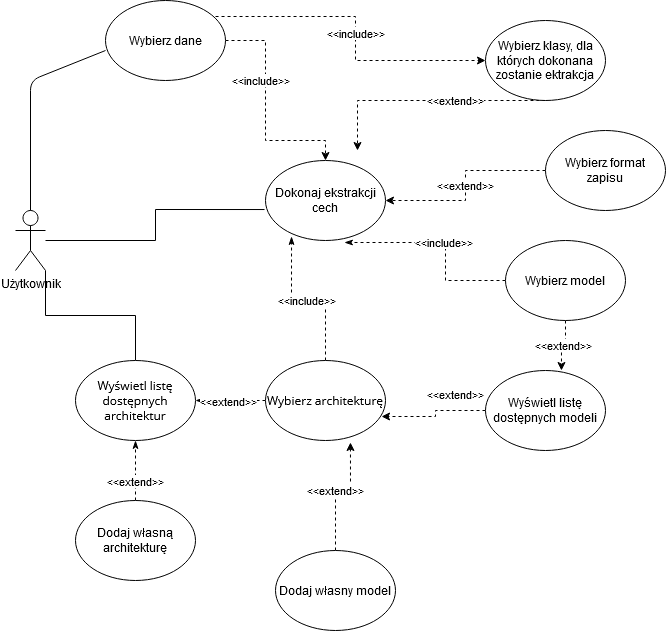
\includegraphics[scale=0.62]{usecase.png}
\caption{Diagram przypadków użycia}
\label{usecase}
\end{figure}

}
\section{Opis narzędzi}

\subsection{Python}
{Python jest wysokopoziomowym językiem, który ze względu na swój rozbudowany system bibliotek oraz zwięzłą i przejrzystą składnię znajduje swoje zastosowanie w wielu dziedzinach, szczególnie tych związanych z uczeniem maszynowym. Python nie wymusza jednego paradygmatu programowania, jak np. C\#, lecz pozwala na użycie różnorodnych technik, takich jak programowanie obietkowe, programowanie strukturalne czy programowanie funkcyjne. Całość tworzonego projektu została stworzona właśnie w tym języku.}
\subsection{Keras i Tensorflow}
{Tensorflow to darmowa i otwartoźródłowa biblioteka, służąca głównie do rozwiązywania zadań z obszaru uczenia maszynowego. Keras służy jako API (ang. \ang{Application Programming Interface}) do biblioteki Tensorflow. Obie te biblioteki zostały użyte do implementacji konwolucyjnej sieci neuronowej. Oferują one możliwość wyborów modelów z już nauczonymi parametrami sieci (np. model VGG16, opisany w podrozdziale \ref{vg}, czy ResNet opisany w \ref{Res}).}
\subsection{Skimage i Imageio}
{Skimage oraz Imageio są blibliotekami języka Python, które umożliwiają łatwe wczytywanie oraz przetwarzanie obrazów. W programie zostały one wykorzystane w implementacji algorytmu wyszukiwania selektywnego, jak i również do zmian rozmiarów obrazów.}
\subsection{Abstract Base Classes}
\label{abc}
{Abstract Base Classes (w skrócie – ABC) to moduł języka Python, który zapewnia infrastrukturę pozwalającą na zdefiniowanie klas abstrakcyjnych. Za jego pomocą tworzona jest abstrakcyjna klasa reprezentująca architekturę sieci. }
\subsection{Tkinter}
{Tkinter to biblioteka umożliwiajaca stworzenia GUI (ang. \ang{Graphical User Interface}) w Pythonie. Została użyta do stworzenia prostego interfejsu graficznego pomiędzy użytkownikiem a programem.}
\subsection{PASCAL VOC}
{W projekcie została wykorzystana baza danych PASCAL VOC 2012\cite{PASCAL} zawierająca 11530 obrazów z wyznaczonymi 27450 regionami zainteresowań, wraz z odpowiadającym im etykietami. Ta baza danych jest publicznie dostępna i przez lata była używana w ramach corocznego konkursu z zadań dotyczących wizji komputerowej.
}

\section{Metodyka pracy nad projektowaniem oraz implementcją}
{Pracę rozpoczęto od ogólnego zapoznania się z dziedziną oraz zrozumienia przedstawionego zagadnienia. Dzięki powszechnie dostępnym źródłom, takim jak artykuły internetowe oraz wykłady udostępniane przez inne uczelnie na serwisach internetowych, szybko pojęto podstawy teoretyczne uczenia maszynowego oraz zasady działania konwolucyjnych sieci neuronowych.}

{Kolejnym krokiem było ustalenie wymagań projektu i wyznaczenie efektu końcowego. W celu lepszej wizualizacji wymagań stworzono również diagram przypadków użycia, ilustrujący przykładowe użycia systemu. Wymagania były następnie sukcesywnie  doprecyzowane, dzięki czemu przedstawiony problem stawał się łatwiejszy do zrozumienia.}

{Następnym krokiem była analiza źródeł odnoszących się już do głównego zagadnienia pracy. Dokonano jej poprzez lekturę publikacji naukowych oraz przeglądu znanych rozwiązań. Zapoznano się również z podobnymi projektami dostępnymi publicznie i ich rozwiązaniami, dzięki czemu uzyskano lepszy punkt odniesienia. Następnie dokonano wyboru odpowiednich narzędzi oraz zapoznano się z ich dokumentacją techniczną.}
{Posiadając tą wiedzę teoretyczną, jasno przedstawiony cel oraz znajomość wybranych narzędzi, przystąpiono do implementacji projektu. Stworzono podstawowy model, do którego następnie dodawane były kolejne funkcjonalości, aż do osiągnięcia wyznaczonego efektu końcowego.}







\chapter{Specyfikacja zewnętrzna}
{W tym rozdziale znajduje się opis specyfikacji zewnętrznej projektu. Opisane zostaną wymaganie sprzętowe, sposób instalacji oraz aktywacji narzędzia. Następnie przedstawiony zostanie sposób obsługi, przykład działania oraz scenariusze korzystania z systemu.}


\section{ Wymagania sprzętowe i programowe}
\subsection{Python }
\begin{itemize}
\item {System operacyjny:}
\begin{itemize}
\item {Windows 7 lub nowszy}
\item {Mac OS X 10.11 lub nowszy, 64-bitowy}
\item {Linux RHEL 6/7, 64-bitowy}
\end{itemize}
\item{Procesor x86 64-bit  (Intel/AMD)}
\item{4GB pamięci RAM}
\item{5GB wolnej przestrzeni dyskowej}
\end{itemize}

\subsection{Tensorflow}
\begin{itemize}
\item{Python 3.5 lub nowszy}
\item {System operacyjny:}
\begin{itemize}
\item {Windows 7 lub nowszy, 64-bitowy}
\item {Mac OS X 10.12.6 lub nowszy, 64-bitowy}
\item {Ubuntu 16.04 lub nowszy, 64-bitowy}
\end{itemize}
\item{Procesor obsługujący instrukcję AVX}

\end{itemize}
 
\section {Sposób instalacji}
\subsection{Python}
{W celu uruchomienia narzędzia należy posiadać zainstalowango Pythona w wersji 3.5 lub nowszej. Można to zrobić poprzez oficjalną stronę internetową, w zakładce Downloads, \url{https://www.python.org/downloads/}. Nalezy pobrać plik odpowiedni dla swojego systemu operacyjnego, a następnie uruchomić go i przejść przez proces instalacji.}
\subsection{Instalacja narzędzia}
{Kod narzędzia należy pobrać z publicznego repozytorium \url{https://github.com/Mikohab450/FeatureExtraction.git}. Można to zrobić na wiele sposobów, pobierając kod bezpośrednio ze strony w formacie .zip, lub klonując repozytorium za pomocą narzędzia git w terminalu  systemowym używając komendy: }

{\lstinline|$ git clone https://github.com/Mikohab450/FeatureExtraction.git| }

\section{Sposób aktywacji}
{Następnie należy zainstalować wszystkie biblioteki potrzebne do działanie programu. Można to zrobić za pomocą wbudowanego w Pythona systemu zarządzania bibliotekami pip. W systemie Windows należy wpisać komendę:}


{\lstinline|C:\ > py -m pip install -r .../FeatureExtraction/requirements.txt| }

{A w systemach Linux oraz Mac OS X:}


{\lstinline|$ python -m pip install -r .../FeatureExtraction/requirements.txt| }

{Gdzie w miejsce \emph{...} należy wpisać ścieżkę, do której narzędzie zostało pobrane. Następnie narzędzie można uruchomić wpisując w terminalu Windowsa}

{\lstinline|C:\ > py .../FeatureExtraction/FeatureExtraction/Main.py| }

{Analogicznie dla pozostałych systemów:}

{\lstinline| $ python .../FeatureExtraction/FeatureExtraction/Main.py| }

{bądź klikając dwukrotnie plik \textbf{Main.py.}}
\section{Przykład działania}
{Po uruchomieniu narzędzia pokaże nam się prosty interfejs, przedstawiony na rysunku \ref{interface}. Za jego pomocą możemy wykorzystywać różne funkcjonalości systemu.}


\begin{figure}[h!]


\centering
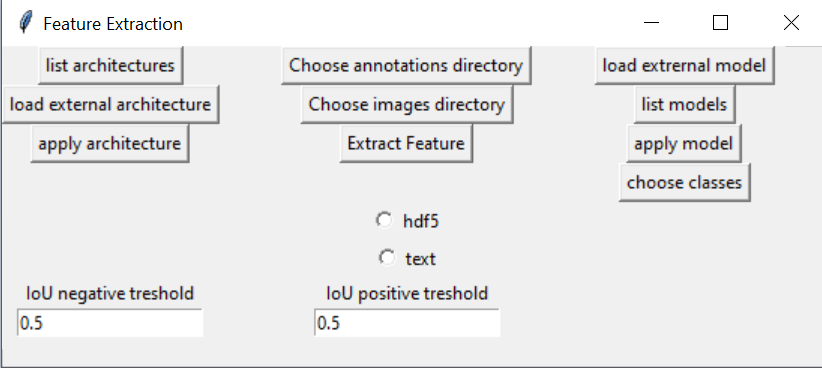
\includegraphics[scale=0.9]{interface.png}
\caption{Interfejs programu}
\label{interface}
\end{figure}

\subsection{Wybór achitektury}
{W celu wybrania architektury sieci należy zaznaczyć architekturę z listy przy pomocy przycisku \emph{list architectures}, a następnie zainicjalizować ją kilkając \emph{apply architecture}. Jeżeli inicjalizacja przebiegła pomyślnie, to wyświetlone zostanie okienko informujące o tym, jaka architektura jest używana. W przeciwnym razie wyświetlona zostanie okienko informujące o wystąpieniu błędu. W przypadku kliknięcia na \emph{apply architecture} bez wcześniejszego wybierania architektury z listy, użyta zostanie domyślna architektura R-CNN. Jeżeli użytkownik chce wybrać architekturę, której nie ma na liście, musi ją najpierw załadować przy pomocy przycisku  \emph{load external architecture}. Po kliknięciu niego będzie miał możliwość wybrania pliku Pythona (modułu), z którego zostanie wczytana architektura. Aby zewnętrzna architektura została wczytana poprawnie, musi spełniać następujące warunki:
\begin{itemize}
\item Architektura musi być klasą dziedziczącą po klasie NetworkArchitecture oraz implementującą wszystkie jej metody.
\item Nazwa pliku oraz nazwa klasy muszą być identyczne.
\end{itemize}
Jeżeli warunki te zostaną spełnione, to po wybraniu pliku pojawi się on na liście architektur i będzie można go wybrać.}
\subsection{Wybór modelu}
{Analogicznie jak przy wyborze architektury, aby wybrać model należy zaznaczyć jeden z listy \emph{list models}, a następnie zainicjalizować przy pomocy \emph{apply model}. Należy pamiętać, że przed wybraniem modelu należy wybrać architekturę. Domyślnym modelem jest VGG16 i to on zostanie użyty jeżeli nie wybierzemy innego modelu z listy. Własny model można załadować klikając \emph{load external model}. Model powinien być w formacie TensorFlow SavedModel lub Keras H5 i mieć wejście o wymiarze 224x224x3.}
\subsection{Wybór i format danych wejściowych}
{Dane wejściowe składają się z dwóch części – folderu ze zdjęciami w dowolnym formacie oraz folderu z odpowiadającymi im adnotacjami. Adnotacje powinny mieć taką samą nazwę pliku (bez rozszerzenia) jak zdjęcie, którego dotyczą. Folder za zdjęciami możemy wybrać klikając w przycisk \emph{Choose images directory}, a folder z adnotacjami poprzez \emph{Choose annotations directory}. 
Na rysunku \ref{example} przedstawiono przykładowe zdjęcie w folderze wejściowym, wzięte z bazy danych PASCAL VOC, a na rysunku \ref{etykieta} pokazano plik zawierający adnotacje do tego zdjęcia.}

\begin{figure}[h!]

\centering
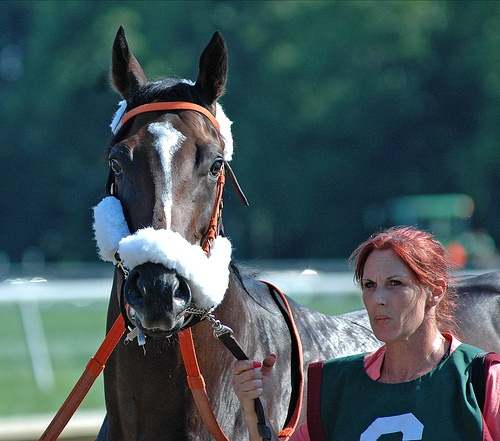
\includegraphics[scale=0.4]{2007_000799.jpg}
\caption{Wybrany obraz z bazy PASCAL VOC}
\label{example}
\end{figure}

\begin{figure}
\centering
\begin{lstlisting}
<annotation>
	<folder>VOC2012</folder>
	<filename>2007_000799.jpg</filename>
	<source>
		<database>The VOC2007 Database</database>
		<annotation>PASCAL VOC2007</annotation>
		<image>flickr</image>
	</source>
	<size>
		<width>500</width>
		<height>441</height>
		<depth>3</depth>
	</size>
	<object>
		<name>horse</name>
		<bndbox>
			<xmin>95</xmin>
			<ymin>23</ymin>
			<xmax>500</xmax>
			<ymax>441</ymax>
		</bndbox>
	</object>
	<object>
		<name>person</name>
		<bndbox>
			<xmin>230</xmin>
			<ymin>225</ymin>
			<xmax>500</xmax>
			<ymax>441</ymax>
		</bndbox>
	</object>
</annotation>

\end{lstlisting}
\caption{Etykieta opisująca rysunek \ref{example}}
\label{etykieta}
\end{figure}
\subsection{Ekstrakcja cech}
{Po wyborze architektury, modelu oraz folderów z danymi wejściowymi należy zaznaczyć format zapisu, a następnie można przystąpić do ektrakcji cech klikając w \emph{Extract features}. Jeżeli którykolwiek z poprzednich kroków nie został wykonany bądź został wykonany niepoprawnie (np. wystąpił błąd podczas jego wykonywania), to ektrakcja się nie wykona i program zwróci stosowny komunikat. Po zakończeniu udanej ekstrakcji program poinformuje o tym użytkownika, wyświetlając okno z informacją \emph{Features saved!}. W zależności od wybranego formatu zapisu, w katalogu głównym programu pojawi się plik \emph{Features.txt} dla formatu tekstowego, lub pliki \emph{annotations.h5} oraz  \emph{activations.h5} dla formatu hdf5. }
\subsection{Format zapisu}
{W przypadku pliku tekstowego, format zapisu wygląda następująco:}

\begin{table}[h!]
\centering
\begin{tabular}{|l|l|l|l|l|l|l|l|}
\hline
Nazwa klasy  & xmin & ymin & xmax & ymax & ID pliku & [IoU] & wektor \\
\hline

\end{tabular}
\end{table}  
{Gdzie \emph{xmin}, \emph{ymin}, \emph{xmax}, \emph{xmax} oznaczają cztery wierzchołki prostokątu, z którego ekstrahowano cechy. W tablicy \ref{cechy} przedstawiono fragment próbki danych wyekstrahowanych ze zdjęcia z rysunku \ref{example}. Ponieważ każdy wektor ma 4096 liczb, pozwolono sobie przestawić tutaj tylko dwie pierwsze.}
{W przypadku zapisu w formacie hdf5 etykiety zapisywane są w pliku \emph{annotations.h5}, a wektory w pliku \emph{activations.h5}.}
\label{format}



\begin{table}[h!]
\centering
\caption{Fragment przykładowych wyektrahowanych danych}
\begin{tabular}{llllllll}
\hline
Nazwa klasy  & xmin & ymin & xmax & ymax & ID pliku & [IoU] & wektor \\
\hline
horse  & 0 & 0 & 223 & 223 & 2007\_000799 & [0.76] & 0.61 2.24 [...]\\
horse  &0 & 0 & 223 & 218 & 2007\_000799 & [ 0.77]  &0.63 2.23 [...]\\
horse &  43 & 55 & 223 & 168 & 2007\_000799 &[0.66] & 0.71 2.06 [...]\\
person &  43 & 101 & 180 & 122 & 2007\_000799 & [0.73] & 0.74 2.33 [...] \\
background & 97 & 157 & 14 & 38 & 2007\_000799 & [0.02, 0.03]& 1.03 1.99 [...]\\
background & 99 & 152 & 12 & 30 & 2007\_000799 &[0.12, 0] & 0.74 2.02[...]\\
\hline
\end{tabular}
\label{cechy}
\end{table}

\subsection{Inne opcje}
\subsubsection{Wybór klas}
{Klikając w przycisk \emph{choose classes} możemy dokonać wyboru klas, które podlegają ekstrakcji. Należy pamiętać, że najpierw należy wybrać folder z etykietami, a dopiero później ograniczać klasy. W przypadku wykonania tych kroków w odwrotnej kolejności wyświetlona lista z klasami będzie pusta.}
\subsubsection{Wybór progów IoU}
{Wpisując liczby w pola \emph{IoU positive treshold} i \emph{IoU negative treshold} można wybrać jaki będzie próg oceny, czy dana etykieta jest lub nie jest obiektem (wiecej o tym w rozdziale \ref{iou}). Wartości te powinny być z przedziału 0-1, logicznym również jest założenie że próg próbek pozytywnych będzie większy lub równy progowi próbek negatywnych, choć nie jest to konieczne. Domyślnie obie zmienne przyjmują wartość 0.5.}


 

\chapter{Specyfikacja wewnętrzna}
{Niniejszy rozdział zawiera opis idei zastosowanego rozwiązania. Opisane zostaną również architektura systemu, użyte klasy, najważniejsze algorytmy oraz komponenty.}
\section{Przedstawienie idei}
{Idea projektu zakładała stworzenie uniwersalnego narzędzia, które zawierałoby w sobie zaimplementowaną architekturę sieci, lecz umożliwiało łatwą rozbudowę o inne architektury. W tym celu połączono mechanikę dziedziczenia oraz dynamicznego ładowania modułów. Do implementacji architektury potrzebne były trzy elementy: odczyt danych, wyznaczenie regionów oraz sieć konwolucyjna. Przy implementacji architektury zadbano o to, aby odczyt danych oraz algorytm selektywnej selekcji służący do wyznaczanie regionów były zaimplementowane jako osobne moduły, dzięki czemu działają niezależnie od reszty rozwiązania.}
\section{Architektura systemu}
{Główną klasą narzędzia klasa \lstinline|View|,  jest odpowiedzialna za wyświetlenie interfejsu graficznego i wykonywanie zadanych funkcjonalności. Działa ona na obiekcie \lstinline|NetworkArchitecture|, który rezprezentuje architekturę sieci, oraz korzysta z modułu \lstinline|DataPrep.py| w celu przetworzenia adnotacji i zapisania ich w odpowiednim formacie.}
\section{Opis najważniejszych klas oraz modułów}
\subsection{NetworkArchitecture.py}
{Moduł zawiera klasę \lstinline|NetworkArchitecture|, która jest klasą abstrakcyjną reprezentującą architekturę sieci. Klasy abstrakcyjne nie są wbudowane w Pythona, dlatego aby osiągnąć ten efekt klasa ta dziedziczy bo klasie \textbf{ABCMeta} z pakietu \textbf{abc} opisanego w podrozdziale \ref{abc}. Klasa ta zawiera następujące metody:}
\begin{itemize}
\item {\lstinline|extract_features_from_image|}
\item{\lstinline|choose_model|}
\item{\lstinline|load_model|}
\end{itemize}
{W celu stworzenia klasy dziedziczacej należy te metody w niej poprawnie zaimplementować. Klasa ta posiada dwa pola \textbf{CNN\_model} oraz \textbf{list\_of\_models}. W pierwszym przechowywany jest sieć konwolucyjna, drugie przechowuje listę dostępnych modeli. Przy implemetacji klasy dziedziczącej należy pamiętać o tym, żeby tych właśnie pól używać przy wczytywaniu i inicjalizaji modeli, ponieważ w przeciwnym razie klasa dziedzicząca nie będzie kompatybilna z resztą programu.}

\subsection{DataPrep.py}
{Moduł ten zawiera funkcje pozwalające na przetworzenie wejściowego folderu z adnotacjami oraz zapisanie tylko tych istotnych adnotacji do pliku csv. Nie zapisujemy wszystkich danych z adnotacji, ponieważ mogą one zawierać również dodatkowe informacje o obiekcie, które są potrzebne do innych zadań (np. do segmentacji czy rozpoznawania akcji). Do zadań klasyfikacji potrzebujemy jedynie nazwę obiektu oraz obwolutę, w której się znajduje, dlatego odczytujemy tylko te dane a następnie zapisujemy je w formacie, z którego łatwo będzie je później odczytać. }
\subsection{SelectiveSearch.py}
{Moduł zawiera funkcję odpowiedzialną na implementację algorytmu wyszukiwania selektywnego, opisanego w podrozdziale \ref{ss}. Do obliczania podobieństwa użyto wizualnego deskryptora nazywanego localnymi wzorami binarnymi (ang.\ang {Local Binary Patterns}), co jest drobym odstępstwem od wcześniej opisanej metody, lecz zasadniczo nie zmienia jej działania. }
\subsection{RCNN.py}
{Moduł zawiera klasę \textbf{RCNN}, która implementuje tą właśnie architekturę sieci, opisaną dokładniej w rozdziale \ref{rcnn}. Dziedziczy ona po klasie \lstinline|NetworkArchitecture|.}
\subsection{View.py}
{W tym module znajduje się klasa \textbf{View.py}, która odpowiada za interfejs graficzny programu. Dziedziczy ona po klasie \lstinline|tkinter.Frame| i jest singletonem, tworzonym i wywoływanym przez główny program.}
\subsection{main.py}
{Moduł służący do uruchomienia projektu. Inicjalizuje instancję klasy \textbf{View} i tworzy główną pętle programu.}

\section{Opis najważniejszych metod i funkcji}
\subsection{Funkcja \lstinline|create_annotations|}
{ Funkcja \lstinline|create_annotations| pokazana na rysunku \ref{dataprep}, znajduje się module \textbf{DataPrep.py} i pobiera jako argument ścieżkę do folderu z adnotacjami, a następnie za pomocą funkcji \lstinline|extract_single_xml_file| odczytuje potrzebne informacje ze wszystkich plików z tego folderu  i zapisuje je w liście, która jest następnie konwertowana do typu \textbf{DataFrame} biblioteki pandas. Ten typ jest przeznaczony do przechowywania danych w postaci tabelarycznej i ma wbudowaną metodę \lstinline|to_csv| umożliwiająca zapis do formatu csv. Używając tej metody zapisujemy potrzebne etykiety w folderze roboczym, aby móc później z nich skorzystać. Funkcja zwraca listę z nazwami wszystkich klas odczytanych z adnotacji.}
\begin{figure}[h!]
\centering
\begin{lstlisting}
def create_annotations(dir_anno):
    df_anno = []
    class_names=[]
    for fnm in os.listdir(dir_anno):  
        if not fnm.startswith('.'):
            tree = ET.parse(os.path.join(dir_anno,fnm))
            row = extract_single_xml_file(tree,class_names)
            row["fileID"] = fnm.split(".")[0]
            df_anno.append(row)
    df_anno = pd.DataFrame(df_anno)
    df_anno.to_csv("etykiety.csv",index=False)
    return class_names}

\end{lstlisting}
\caption{Definicja funkcji \lstinline|create_annotations|}
\label{dataprep}
\end{figure}
\subsection{Funkcja \lstinline|get_region_proposal|}
 Funkcja \lstinline|get_region_proposal|, która znajduje się w module \textbf{SelectiveSearch}, pokazana jest na rysunku \ref{search}. Przyjmuje ona jako argument wejściowy obraz, dla którego regiony maja być wyznaczone. Zwraca listę słowników zawierających wyznaczone regiony.}
\begin{figure}[h!]
\centering
\begin{lstlisting}
def get_region_proposal(img_8bit,min_size = 500):
    img = image_segmentation(img_8bit,min_size = min_size)
    R  = extract_region(img)    
    tex_grad = calc_texture_gradient(img)
    hsv = calc_hsv(img)
    R  = augment_regions_with_histogram_info(tex_grad, img, R,hsv,tex_grad)
    del tex_grad, hsv
    neighbours = extract_neighbours(R)
    S  = calculate_similarlity(img,neighbours)
    regions = merge_regions_in_order(S,R,imsize = img.shape[0] * img.shape[1])
    no_duplicates  = remove_duplicates(regions)
    return(no_duplicates)
\end{lstlisting}
\caption{Definicja funkcji  \lstinline|get_region_proposal|}
\label{search}
\end{figure}

\subsection{Metoda \lstinline|warp_and_create_cnn_feature|}
{Metoda te zdefiniowana jest w klasie \textbf{RCNN} i oblicza cechy głębokie dla otrzymanej listy obrazów \textbf{image}. Dla każdego obrazu z listy najpierw zmienia jego rozmiar za pomocą metody \lstinline|warp| tak, aby jego wymiary były kompatybilne z wejściem sieci konwolucyjnem. Obraz jest przepuszczany przez sieć poprzez użycie wbudowanej metody \textbf{predict}, która operuje na modelu sieci neuronowej, który jest obiekem klasy \textbf{Model} z biblioteki \emph{Keras}. }
\begin{figure}[h!]
\centering
\begin{lstlisting}
    def warp_and_create_cnn_feature(self,image):
        for irow in range(len(image)):
            image[irow] = self.warp(image[irow],self.warped_size)
        image = np.array(image)
        feature = self.CNN_model.predict(image)
        return(feature)
\end{lstlisting}
\caption{Defnicja funkcji \lstinline|warp_and_create_cnn_feature||}
\label{warp}
\end{figure}
\subsection{Metoda \lstinline|extract_features_from_image|}
{Metoda \lstinline|extract_features_from_image| działa na obiekcie klasy \textbf{RCNN} i służy do wyznaczenia odpowiednich regionów z odpowiadającymi im adnotacjami, a następnie wyliczenia dla niech wektorów cech. Funkcja przyjmuje  następujące parametry:}
\begin{itemize}
\item {\textbf{img\_dir} – ścieżka do folderu zawierającego zdjęcia.}
\item {\textbf{classes} – słownik z nazwami klas, dla których dokonana ma być ektrakcja. Każda nazwa klasy jest kluczem, której odpowiada wartość typu \textbf{tkinter.BooleanVar}}
\item {\textbf{IoU\_cutoff\_object} – wartość współczynnika IoU, powyżej której etykieta ma być zakwalifkowana jako obiekt. Domyślnie przyjmuje wartość 0.5.}
\item {\textbf{IoU\_cutoff\_not\_object} – wartość współczynnika IoU, poniżej której etykieta ma być zakwalifkowana jako tło. Domyślnie przyjmuje wartość 0.5.}
\end{itemize}

{Metoda ta odczytuje etykiety z pliku \emph{etykiety.csv} zapisanego w folderze roboczym. Następnie iteruje po kolejnych etykietach każdego obrazu, znajdując odpowiadajacy obraz w folderze \textbf{img\_dir}. W celu przyspieszenia obliczeń każdy obraz jest skalowany do mniejszych rozmiarów przy pomocy funkcji \lstinline|warp|. Następnie obliczane są propozycje regionów, po czym rozpoczyna się iterację po wszystkich obiektach znajdujących się w obrazie. Używając zmiennej \textbf{classes} sprawdza się, czy obiekt powinien być brany pod uwagę przy ektrakcji. Jeżeli nazwie obiektu odpowiada wartość \emph{False}, to pętla jest przerywana i następuje przejscie do kolejnego obiektu. W przeciwnym wypadku obliczenia są kontynuowane. Ponieważ obraz jest przeskalowany, to wymiary prostokątów zawierajacych obiekty, które zostały odczytane w pliku csv są niewłaściwe i należy je również przeskalować. Po przeskalowaniu trzymujemy zmienne \emph{true\_xmin}, \emph{true\_ymin}, \emph{true\_xmax}, \emph{true\_ymax}, które opisują cztery wierzchołki prostokąta w zmienionym już rozmiarze. Następnie iterujemy po wszystkich propozycjach regionów, obliczając wartość współczynnika IoU za pomocą funkcji \lstinline|get_IOU|, poczym  porównujemy ten współczynnik do zmiennych \textbf{IoU\_cutoff\_object} oraz \textbf{IoU\_cutoff\_not\_object}. Na podstawie tych porównań umieszczamy wierzchołki regionu wraz z nazwą klasy, obliczonym współczynnikiem IoU oraz nazwą akurat przetwarzanego obrazu do listy \textbf{info\_pos} dla próbek pozytywnych, lub \textbf{info\_neg} dla negatywnych. Dodatkowo na podstawie regionu wyznaczany jest fragment obrazu, który zapisywany jest odpowiednio w \textbf{image\_pos} badź \textbf{image\_neg}. Po zakończeniu wszystkich iteracji łączone są listy \textbf{image\_pos} z \textbf{image\_neg} oraz \textbf{info\_pos} z \textbf{info\_neg}. Następnie połączone listy z regionami są przekazywane do funkcji \lstinline|warp_and_create_cnn_feature|, która wylicza dla nich cechy. Funkcja zwraca krotkę zawierajacą stworzone etykiety oraz odpowiadające im cechy.




\chapter{Weryfikacja i walidacja}
{Podczas tworzenia projektu każdy moduł i funkcjonalość były systematycznie testowane pod względem poprawności funkcjonowania.}
\subsubsection{Moduły DataPrep oraz SelectiveSearch}
{Obydwa te moduły zostały stworzone na początku pracy nad narzędziem i były one testowane jeszcze przed przejściem do następnych etapów pracy. W celu weryfikacji poprawności ich działania, wizualizowano rezultaty działań, dzieki czemu można było zobaczyć, czy otrzymane wyniki pokrywają się z oczekiwaniami. Na rysunku \ref{wiz} pokazano działanie algorytmu segmentacji metodą Felzenszwalba, a na rysunku \ref{regions} wyświetlono regiony wyznaczone przez algorytm wyszukiwania selektywnego. Jednym z problemów napotkanym w tym obszarze pracy było wyznaczania kilku regionów o identycznych wymiarach. Nie był to co prawda błąd uniemożliwiający działanie narzędzia, lecz raczej niechciane zachowanie, które zlikwidowano poprzez dodanie funkcji usuwającej duplikaty z listy regionów.
}
\begin{figure}[h!]


\centering
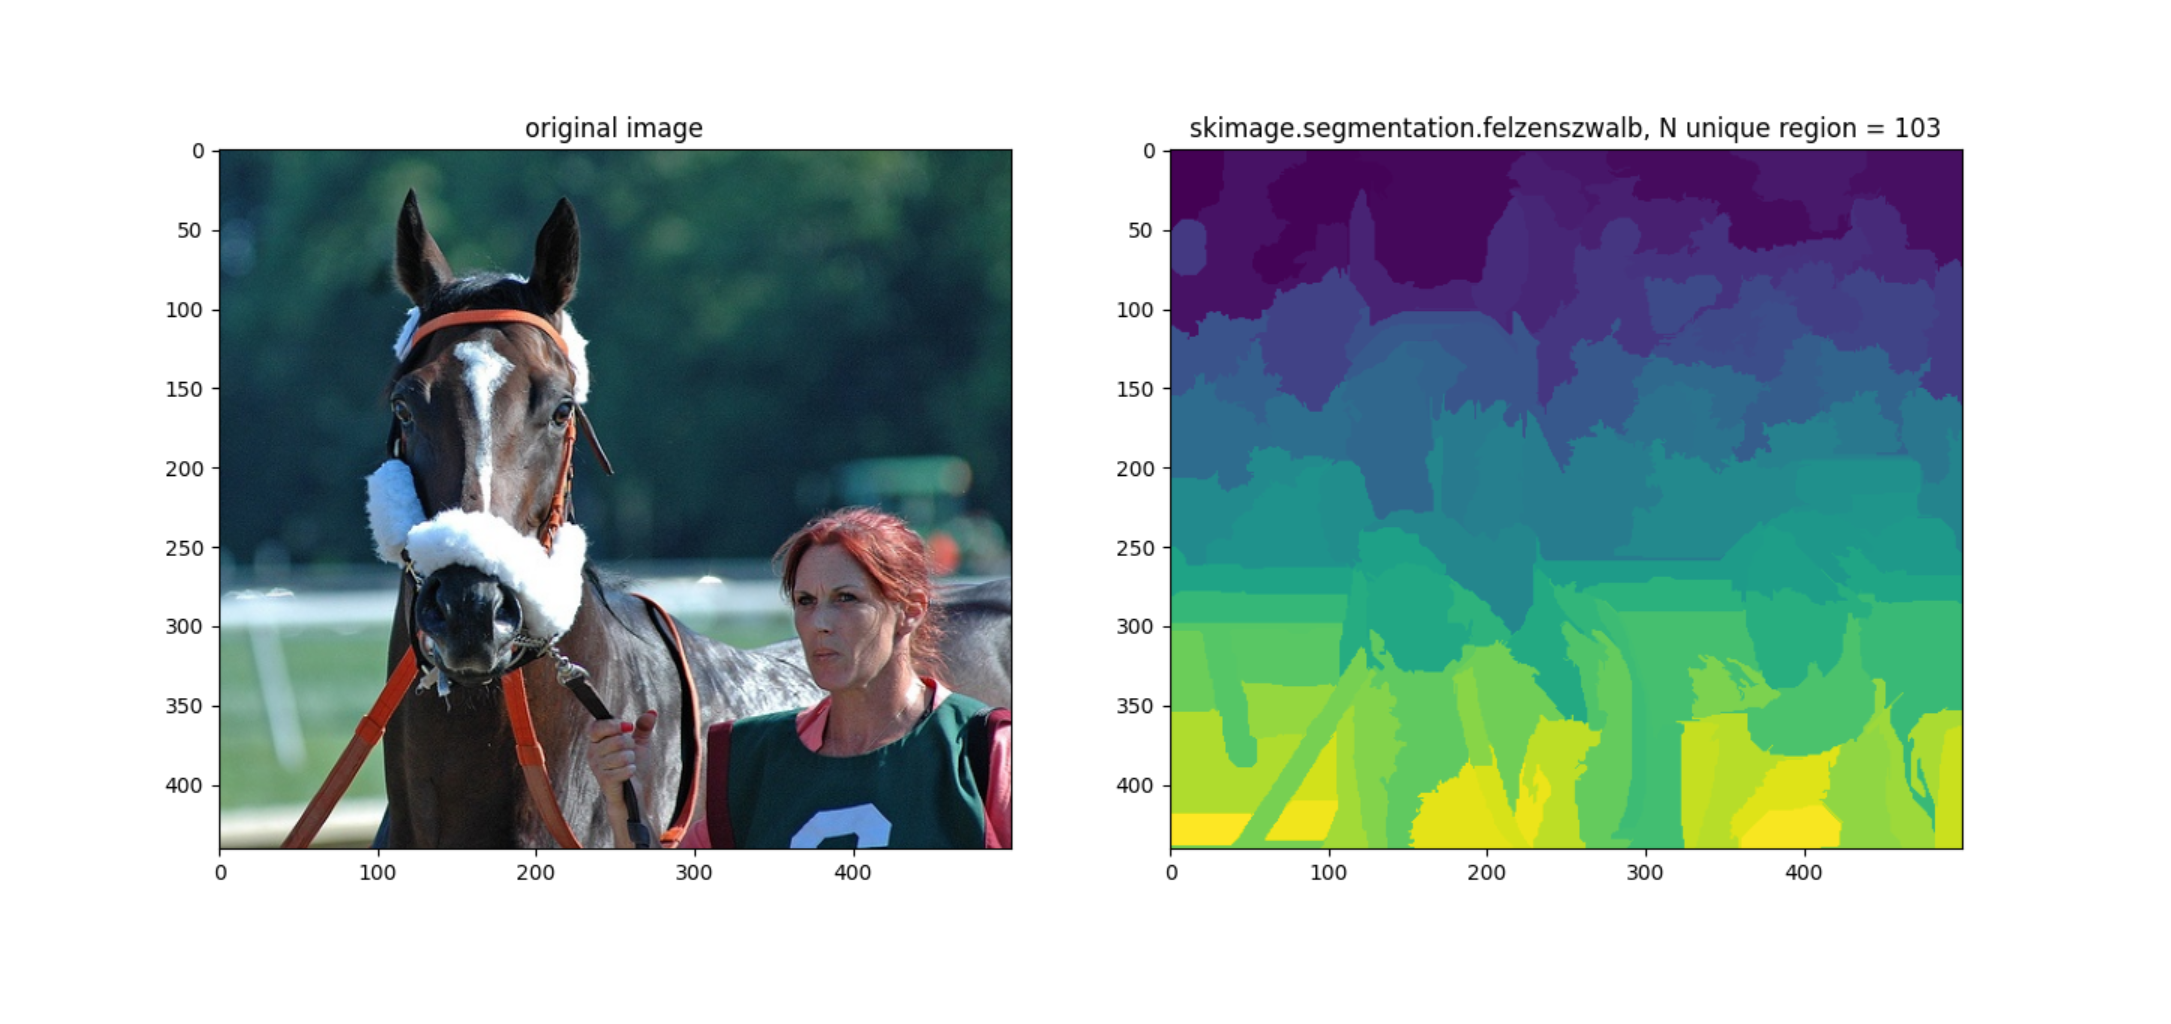
\includegraphics[scale=0.3]{example.png}
\caption{Wizualizacja segmentacji metodą Felzenszwalba.}
\label{wiz}
\end{figure}



\begin{figure}[h!]


\centering
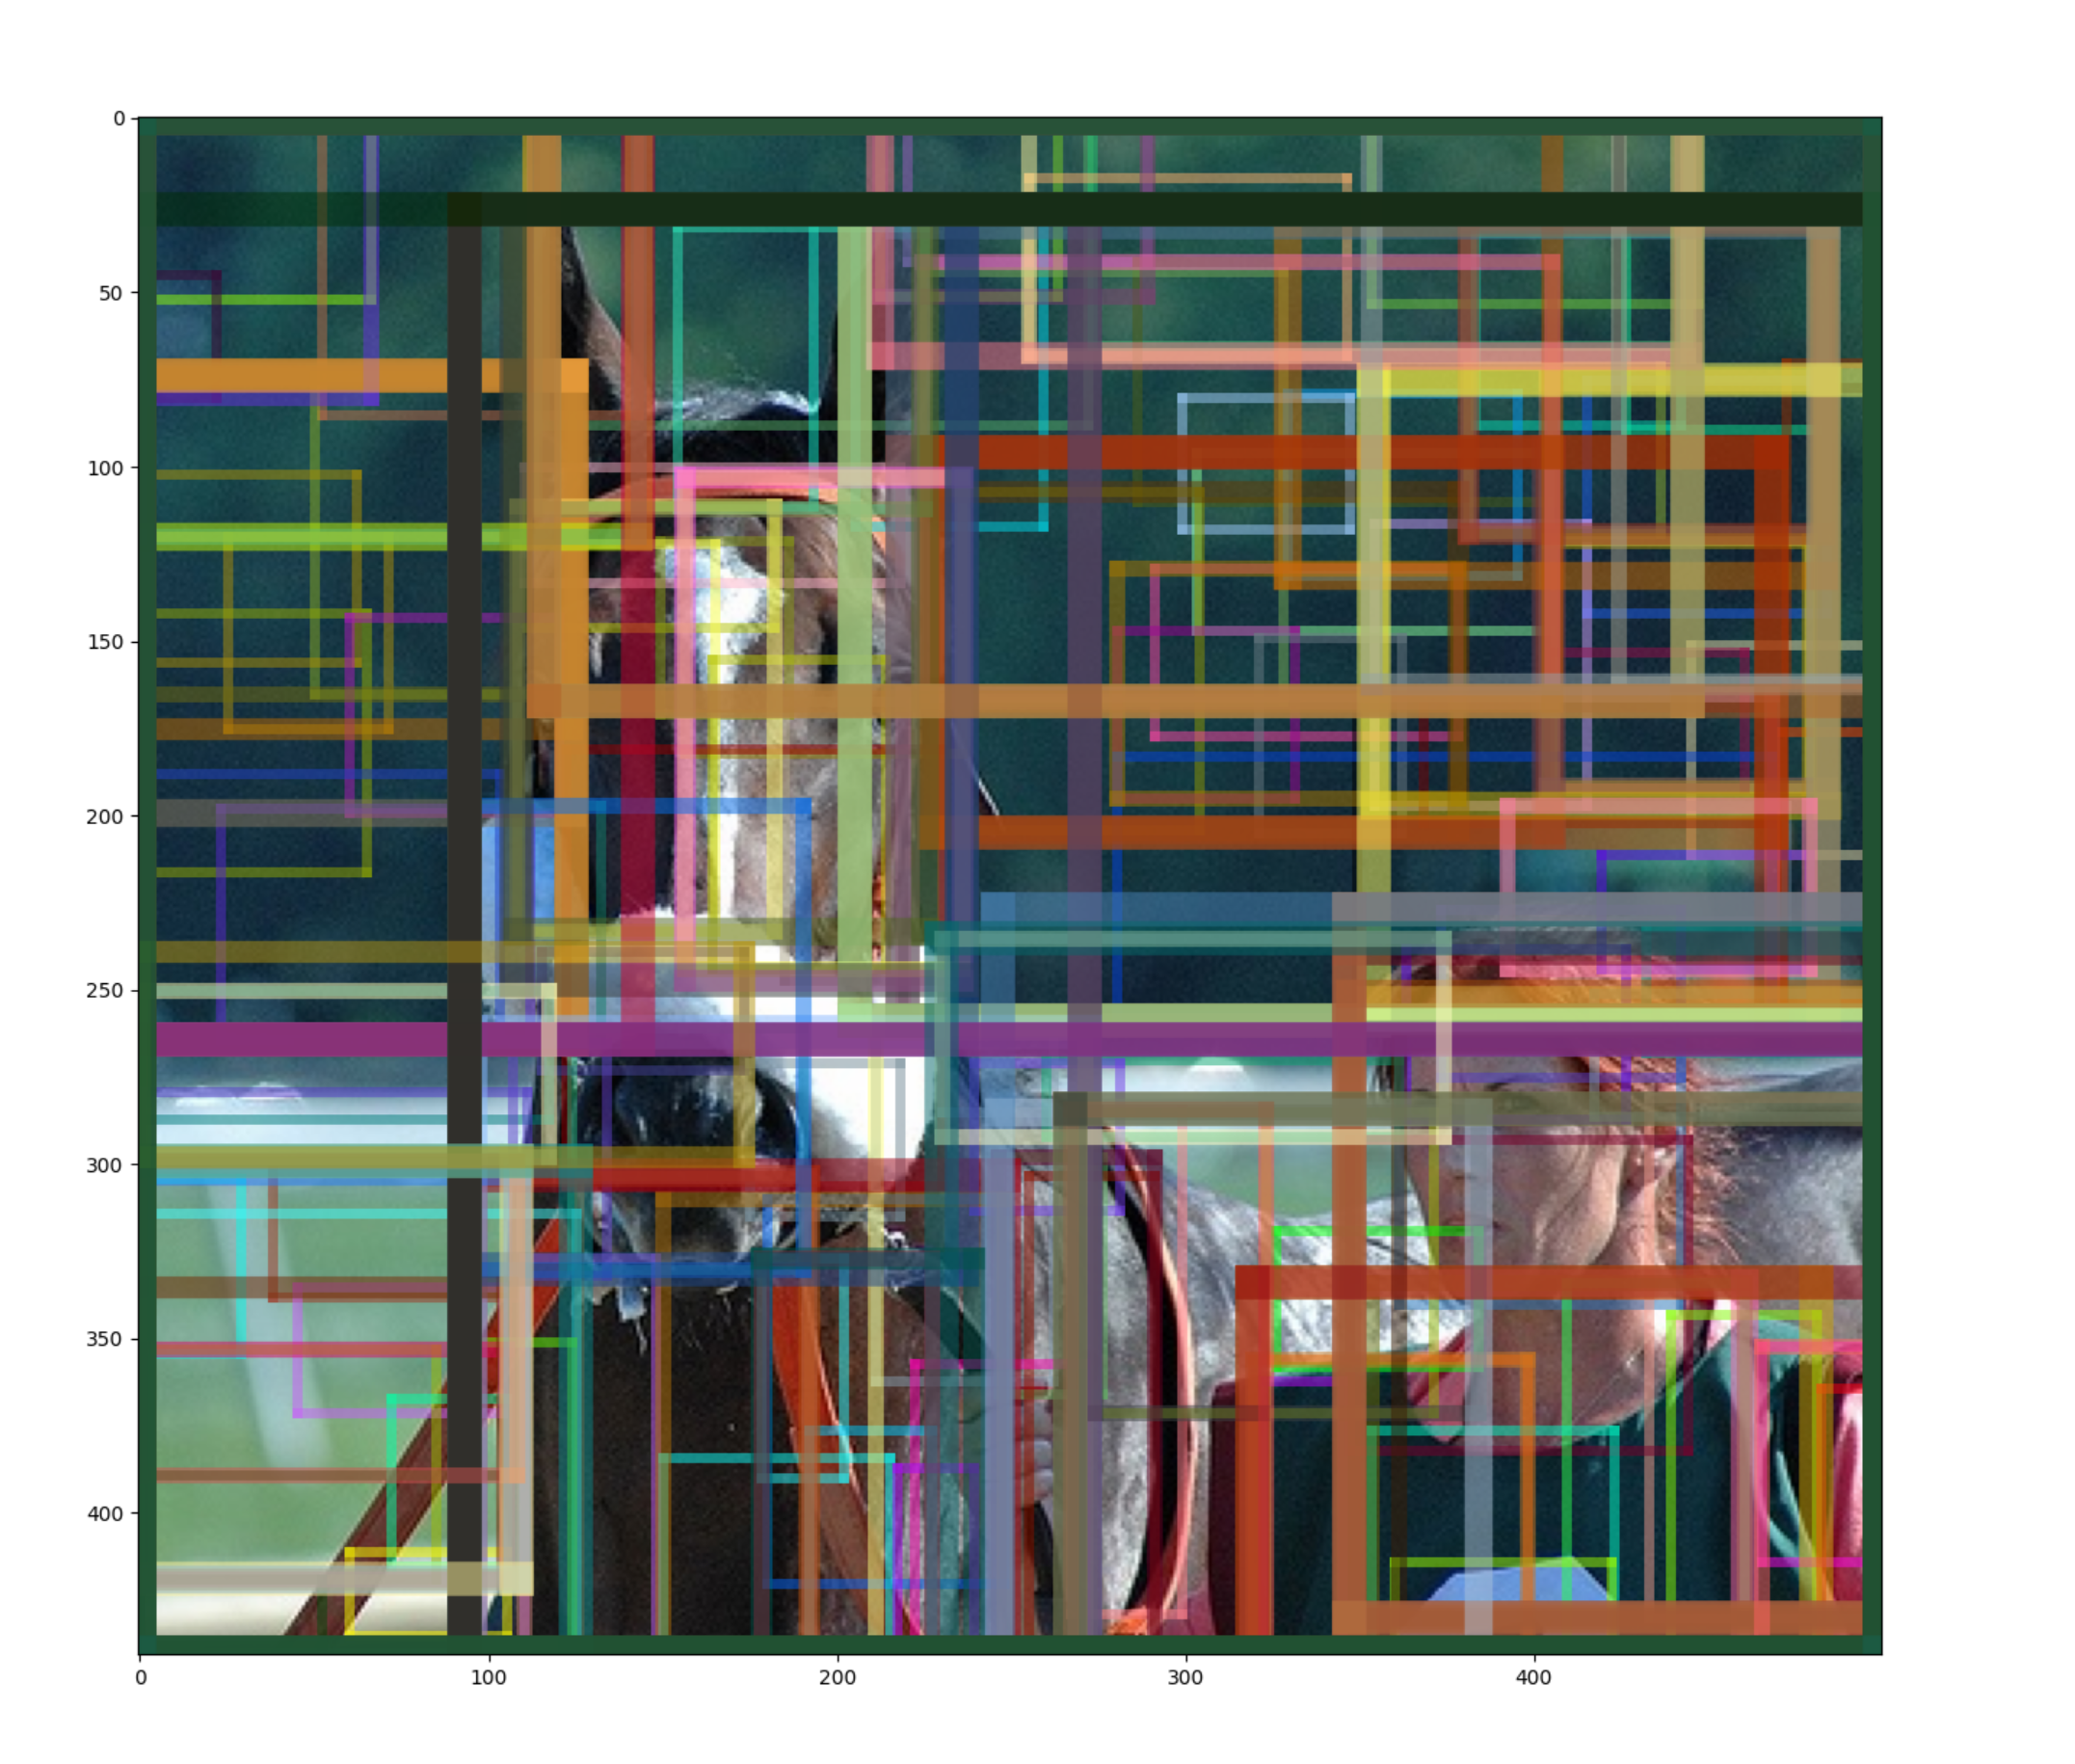
\includegraphics[scale=0.2]{example2.png}
\caption{Wizualizacja wyznaczonych regionów.}
\label{regions}
\end{figure}

\subsubsection{Moduł View}
{W celu przetestowania funkcjonalności dodawania zewnętrznych architektur stworzono testową klasę \textbf{exampleModel}. Następnie sprawdzono, czy po wybraniu pliku z tą klasą moduł jest ładowany poprawnie, czy jest ona wyświetlana na liście architektur oraz czy po zainicjalizowaniu jej jest tworzona instancja jej klasy. Podczas testowania tego elementu zauważono nieoczekiwane zachowanie systemu – w przypadku wyjścia z okna dialogowego podczas wczytywania pliku system pomimo tego, że żaden plik nie został wybrany, próbował otworzyć plik o pustej nazwie, co powodowało błąd. Dodanie warunku sprawdzajacego, czy jakiś plik został wybrany, rozwiązało problem.}

{Podczas testowania funkcjonalości wyświetlania list napotkano na kolejną słabość systemu. Każde naciśnięcie przycisku wyświetlającego listę otwierało nowe okno z listą, można więc było otwierać nieograniczoną ilość okien. Dodatkowo w przypadku wielu otwartych okien z listami próba wybrania elementu z jednej z nich kończyła się błędem sytemu. Problem rozwiązano poprzez ograniczenie ilości wyświetlanych okien, tak aby tylko jedno okno z listą mogło być otwarte w danym momencie. }

{Kolejnym problem napotkano podczas zapisu danych w formacie hdf5. Okazało się, że format ten używa kodowania UTF-8 dla zmiennych typu \emph{String}, podczas gdy Python używa UTF-32. Ta niekompatybilność okazała się być bardzo frustrująca, jednak udało się ją rozwiązać poprzez ustalenie użycia specjalnego typu z biblioteki hdf5 oraz podział etykiet i aktywacji na osobne pliki.}

\section{Wyniki eksperymentalne}
{W celu oszacowania szybkości działania narzędzia oraz ilości zużywanej pamięci, przeprowadzono szereg testów dla różnych ilości danych wejściowych. Wybrano losowo ze zbioru danych PASCAL VOC określoną liczbę zdjeć, a następnie zmierzono czas wykonywania algorytmu wyszukiwania selektywnego ($t_1$), ekstrakcji cech  ($t_2$), zapisu do pliku ($ t_3$) oraz ich sumę  ($ t_c$). Zmierzono również ilość pamięci, która była w użyciu przez proces podczas zakończenia obliczeń. Wyniki przedstawiono w tabeli \ref{wyniki}. }
{Można zaobserwować, że czas zapisu ($t_3$) w formacie hdf5 jest szybszy od zapisu w formacie tekstowym. Nie jest to zaskoczeniem, ponieważ format hdf5 został stworzony specjalnie do efektywnego operowania na dużych zbiorach danych, i wykonuje takie operacje bardziej optymalnie. Nie udało się niestety przeprowadzić badań nad większą liczbą obrazów, ponieważ ilość dostępnej pamięci była niewystarczająca. Jak można łatwo policzyć, wyznaczając ok. 400 regionów na jeden obraz, każdy region o wymiarach $224\times224\times3$, otrzymujemy dla pięciu obrazów ponad 300 milionów liczb. Doliczyć do tego należy jeszcze sieć neuronową, która również zawiera mnóstwo parametrów (użyty w tym przykładzie VGG16 zajmuje ponad 400MB) i otrzymujemy ogromne zapotrzebowanie na pamięć. Warto zaznaczyć, że wszystkie obliczenia były dokonywane tutaj za pomocą technologii CUDA – możliwość zrównoleglenia obliczeń na karcie graficznej pozwala skrócić czas wykonywania obliczeń ponad 6-krotnie w porównaniu do wykonywania ich na zwykłym procesorze.}
\begin{table}[h!]
\centering
\caption{Czas wykonania w sekundach oraz zużycie pamięci w zależności od liczby obrazów oraz formatu zapisu. Do badań użyto modelu VGG16.}
\label{wyniki}
\begin{tabular}{|c|ccccccc|}
\toprule	
	$Obrazy $ &Format &       $t_1$ & $t_2$ & $t_3$ & $t_c$& $\bar{t_c}$ & Pamięć(GB) \\
\midrule  

	       \multirow{4}*{1 }  
	       					& \multirow{2}*{text} 
	       					  & 0.73 & 11.66 & 3.18 &  14.84 &  \multirow{2}*{15.86} &  1.235  \\
	       					  & &  0.98 & 13.24 & 3.64 &  16.88 &  &1.30  \\
	       					  \cline{2-8}
	       					  & \multirow{2}*{hdf5} 
	       					  & 0.87 & 10.74 & 1.01 &  11.75& \multirow{2}*{11.60} & 1.36  \\
	       					  & &  0.72 & 10.59& 0.86 &  11.45 &  &0.96 \\
	       					   \cline{1-8}
		 \multirow{4}*{ 2}  
		 	& \multirow{2}*{text} 
	       					  & 0.93 & 17.25 & 4.35 & 21.60 &\multirow{2}*{21.06} & 0.83
 \\
	       					  & &  1.01 & 16.02 & 4.50 &  20.52 & & 0.91
  \\	 \cline{2-8}
	       					  & \multirow{2}*{hdf5} 
	       					  & 1.02& 15.12 & 0.91 &  16.33 & \multirow{2}*{16.20} & 0.71
 \\
	       					  & &  0.93  & 14.45 & 0.71 &  16.06& & 1.12
 \\ 	\cline{1-8}
	        \multirow{4}*{ 3}     		& \multirow{2}*{text} 
	       					  & 3.98 & 21.77 & 8.51 &30.28 & \multirow{2}*{35.38} & 0.93  \\
	       					  	       					  & &  2.86& 31.4 &9.00 &  40.48 &  &1.36 \\
	       					  	       					   \cline{2-7}
	       					  & \multirow{2}*{hdf5} 
	       					  	       					  & 2.80& 50.9 & 3.30 &  54.23 &\multirow{2}*{54.57} &  1.37  \\
	       					  & &  2.91 & 51.2 & 3.67 &  54.90&  &1.39 \\ 
	       					   \cline{1-8}
	\multirow{4}*{ 5}  
 		& \multirow{2}*{text} 
	       					  & 4.31& 50.4 & 12.28 &  62.71& \multirow{2}*{76.40} & 1.56  \\
	       					  & &  5.15& 59.16 & 30.93&  90.08&  &1.81  \\
	       					   \cline{2-8}
	       					  & \multirow{2}*{hdf5} 
	       					  	       					  & 4.65 & 66.98 & 5.86&  72.84 &\multirow{2}*{77.27} &  1.73  \\
							 & &  4.82 & 75.88 & 5.83 & 81.70 &  &1.64  \\


\bottomrule
\end{tabular}
\end{table}  



\chapter{Podsumowanie i wnioski}
{W ramach pracy udało się stworzyć narzędzie do ekstrakcji cech głębokich za pomocą konwolucyjnych sieci neuronowych, wraz z zaimplementowaną architekturą R-CNN. Zrealizowano wszystkie wymagania funkcjonalne oraz niefunkcjonalne, które zostały postawione na początku pracy. W toku pracy wprowadzono również nowe funkcjonalności, których nie były uwzględnione przy etapie planowania. Dodanie takich funkcjonalności było zazwyczaj podyktowane podniesieniem komfortu korzystania z narzędzia oraz zapewnieniem użytkownikowi większej kontroli nad działaniem algorytmu.}

{Jednym z ważnych aspektów, który miano na uwadze podczas tworzenia projektu była jego uniwersalność i możliwość dostosowania pod własne preferencje. Narzędzie działa dla dowolnych danych, oferuje możliwość wybrania jednego z kilku znanych modeli sieci, jak i wybór własnej sieci użytkownika. Dodatkowo dzięki mechanizmowi wczytywania architektur z pliku możliwa będzie jego dalsza rozbudowa.}

{Początkowy etap tworzenia aplikacji okazał się być najbardziej wymagający. Zdobycie odpowiedniej wiedzy teoretycznej z tak obszernego działu nie było łatwe, a po uzyskaniu jej problemem był brak doświadczenia w praktycznym wykorzystaniu tej wiedzy. Mimo, że wybrany język programowania i technologie nie były zupełnie obce, to niektóre bardziej złożone mechanizmy oraz zachowania wymagały lepszego zapoznania się. W takich przypadkach pomocna okazała się oficjalna dokumentacja zarówno Pythona, jak i poszczególnych bibliotek.}

{Tworzenie aplikacji nie obyło się bez pewnych komplikacji. Aby poprawnie przetestować jakieś rozwiązanie, często trzeba było czekać kilka minut, aż program wykona obliczenia i przejdzie do newralgicznej części kodu. Aby to zminimanizować, podczas pracy działano na bardzo małych próbkach danych, dzięki czemu czas oczekiwania się skracał.}

{Stworzone narzędzie było ciekawym, angażującym oraz wymagajacym projektem. W celu jego realizacji poznano najnowsze odkrycia w dziedzinie wizji komputerowej oraz użyto popularnych technologii, które zyskują coraz to większe wpływy na rozwój techniki.}



 
 

%%%%%%%%%%%%%%%%%%%%%%%%%%%%
\backmatter 
\stepcounter{stronyPozaNumeracja}
\pagenumbering{Roman}
\setcounter{page}{\value{stronyPozaNumeracja}}
\pagestyle{tylkoNumeryStron}
%%%%%%%%%%%%%%%%%%%%%%%%%%%%%
 
\bibliographystyle{ieeetr}
\bibliography{bibliografia}

%%%%%%%%%%%%%%%%%%%%%%%%%%%%%



\begin{appendices}
 

\chapter*{Spis skrótów i symboli}

\begin{description}
\item[RoI] Region zainteresowań  (ang. \ang{Region of Interest})
\item[IoU] Przecięcie nad połączeniem (ang. \ang{Intersection over Union})
\item[CUDA] \ang{Compute Unified Device Architecture}
\item[ILSVRC] ImageNet Large Scale Visual Recognition Challenge
\item[API] Interfejs Programowania Aplikacji(ang. \ang{Application Programming Interface})
\item[GUI] Graficzny Interfejs Użytkownika (ang. \ang{Graphical User Interface})
\item[PASCAL] Pattern Analysis, Statistical Modelling and Computational Learning
\item[PASCAL VOC] PASCAL Visual Object Classes
\item[YOLO] \ang{You Only Look Once}
\end{description}


\chapter*{Załącznik A: Wybrane fragmenty kodu źródłowego}

\begin{lstlisting}
 def extract_features_from_image(self,img_dir,classes,IoU_cutoff_object = 0.5,IoU_cutoff_not_object = 0.5):        
        anno = pd.read_csv("etykiety.csv")        
        image_pos,image_neg, info_pos,info_neg  = [],[],[],[]
        for irow in range(anno.shape[0]):
            row  = anno.iloc[irow,:]
            path = os.path.join(img_dir,row["fileID"] + ".jpg")
            image  = imageio.imread(path)
            orig_h, orig_w, _ = image.shape          
            img = self.warp(image,self.warped_size)
            orig_nh, orig_nw, _ = img.shape
            regions = ss.get_region_proposal(img,min_size=50)[::-1]
            for ibb in range(row["nobj"]): 
                name = row["bbx_{}_name".format(ibb)]
                if not classes[name].get():
                    break;       
                multx, multy  = orig_nw/orig_w, orig_nh/orig_h 
                true_xmin     = row["bbx_{}_xmin".format(ibb)]*multx
                true_ymin     = row["bbx_{}_ymin".format(ibb)]*multy
                true_xmax     = row["bbx_{}_xmax".format(ibb)]*multx
                true_ymax     = row["bbx_{}_ymax".format(ibb)]*multy       
                object_found_TF = 0
                _image1 = None
                for r in regions:                    
                    prpl_xmin, prpl_ymin, prpl_width, prpl_height = r["rect"]
                    IoU = ss.get_IOU(prpl_xmin, prpl_ymin, prpl_xmin + prpl_width, prpl_ymin + prpl_height,
                                     true_xmin, true_ymin, true_xmax, true_ymax)
                    img_bb = np.array(img[prpl_ymin:prpl_ymin + prpl_height,
                                          prpl_xmin:prpl_xmin + prpl_width])            
                    if IoU > IoU_cutoff_object:
                        found_object=[name, prpl_xmin, prpl_ymin, prpl_width, prpl_height,row["fileID"]]
                        info_pos.append(found_object)#.encode('utf-8')
                        image_pos.append(img_bb)
                        background = ["background", prpl_xmin, prpl_ymin, prpl_width, prpl_height,row["fileID"]]
                        if background in info_neg: 
                                back_indx=info_neg.index(background)#if the regions figures as the background sample, delete it
                                del info_neg[back_indx] #from both annotations
                                del image_neg[back_indx] #and images list                                                                                    
                    elif IoU < IoU_cutoff_not_object:
                        background=["background", prpl_xmin, prpl_ymin, prpl_width, prpl_height,row["fileID"]]
                        if background not in info_neg:
                            info_neg.append(background)
                            image_neg.append(img_bb)
        images = image_pos+image_neg
        infos= np.array(info_pos+info_neg,dtype=h5py.string_dtype())
        features = self.warp_and_create_cnn_feature(images)
        return  (infos,features)
       
\end{lstlisting}
 

\chapter*{Zawartość dołączonej płyty}

Do pracy dołączona jest płyta CD z~następującą zawartością:
\begin{itemize}
\item praca (źródła \LaTeX owe i końcowa wersja w \texttt{pdf}),
\item źródła programu,
\item dane testowe.
\end{itemize}

\listoffigures
\listoftables
	
\end{appendices}


\end{document}


%% Finis coronat opus.